\documentclass[../main.tex]{subfiles}
\graphicspath{{\subfix{../images/}}}
\begin{document}

\chapter{System analysis and design}
\section{Proposed software}
\subsection{Functional requirements}

\begin{table}[!ht]
    \caption{functional requirements}  
    \centering
    \begin{tabular}{|c|l|}
       \hline
       Requirement \# & Requirement definition\\
\hline
REQ00 & The game will be in 2D. \\
\hline
REQ01 & The game will include a collection of electric components. \\
\hline
REQ02 & The player will be able to drag and drop the components. \\
\hline
REQ03 & The game will feature puzzle-style levels.\\
\hline
REQ04 & Each level will have a goal to complete. \\
\hline
REQ05 & The player will progress by finishing levels. \\
\hline
REQ06 & The levels will follow a hierarchical tree-structure. \\
\hline
REQ07 & The level-topics will follow standard electric circuit introductory \\
& curriculum structure. \\
\hline
REQ08 & The game must be able to simulate electric circuits. \\
       \hline
       \end{tabular}
    \label{fuctional}
\end{table}

\subsection{Non-functional requirements}

\begin{table}[!ht]
    \caption{functional requirements}  
    \centering
    \begin{tabular}{|c|l|}
       \hline
       Requirement \# & Requirement definition\\
\hline
REQ00 & The game should provide descriptive messages on failure. \\
\hline
REQ01 & The game must be fun. \\
\hline
REQ02 & The game could feature illustrative animations. \\
\hline
REQ03 & The game must feature a user-friendly interface.\\
\hline
REQ04 & The game should be suitable for: electric circuits students. \\
\hline
REQ05 & The game must be educational
\\
\hline
REQ06 & The game should be suitable for: electric circuits hobbyists.\\
\hline
REQ07 & The game should be suitable for: anyone that enjoys puzzle games.\\

       \hline
       \end{tabular}
    \label{non_functional}
\end{table}
\newpage
\section{System Architecture}

The game will run on the unity game engine utilising a lot of its features. As for the simulation of the circuits the we will use the C\# library SpiceSharp. SpiceSharp is a circuits simulation library that is compatible with the Berkeley Spice simulator. The player will interact with the game through its user interface, those interactions could be navigational interactions to transition from one menu or scene to another, or they could be gameplay interactions when playing a level. Then in order to complete a level the player needs to achieve some goals that are introduced at the beginning of the level. The circuits submitted by the player is then simulated using SpiceSharp and the results are sent back to the game, the game then decides whether the goals were achieved or not.
\begin{figure}[ht]
\centering
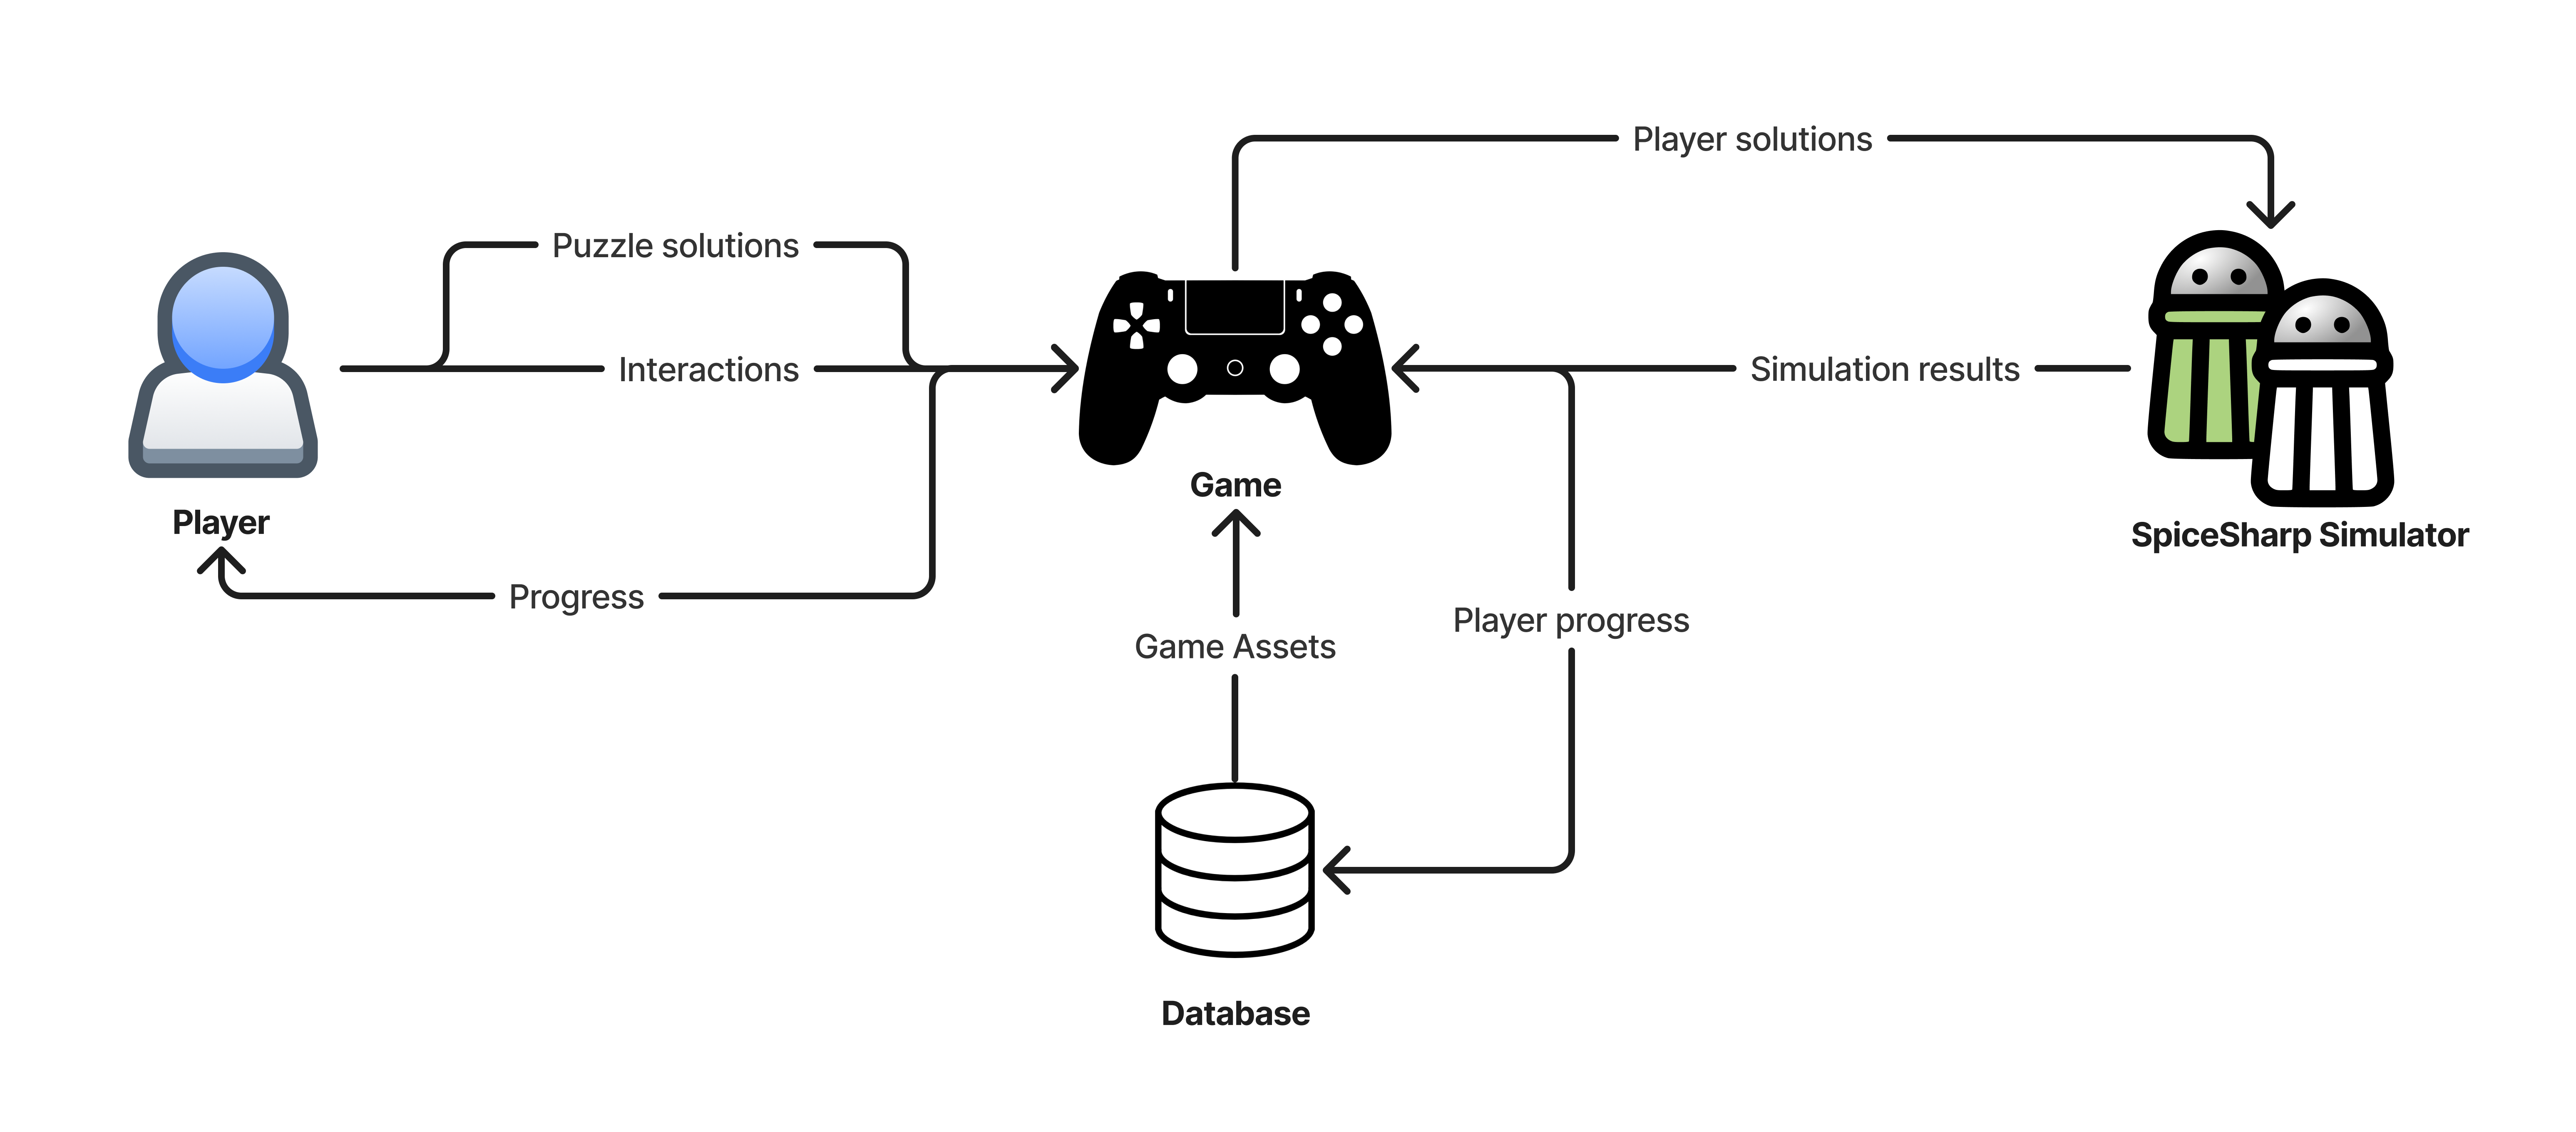
\includegraphics[scale=0.14]{images/chapter3/System Design & Architecture.png}
\caption{System Design \& Architecture.png}
\label{System Design and  Architecture.png}
\end{figure}

\section{system analysis}

\subsection{Context Diagram}
\begin{figure}[ht]
\centering
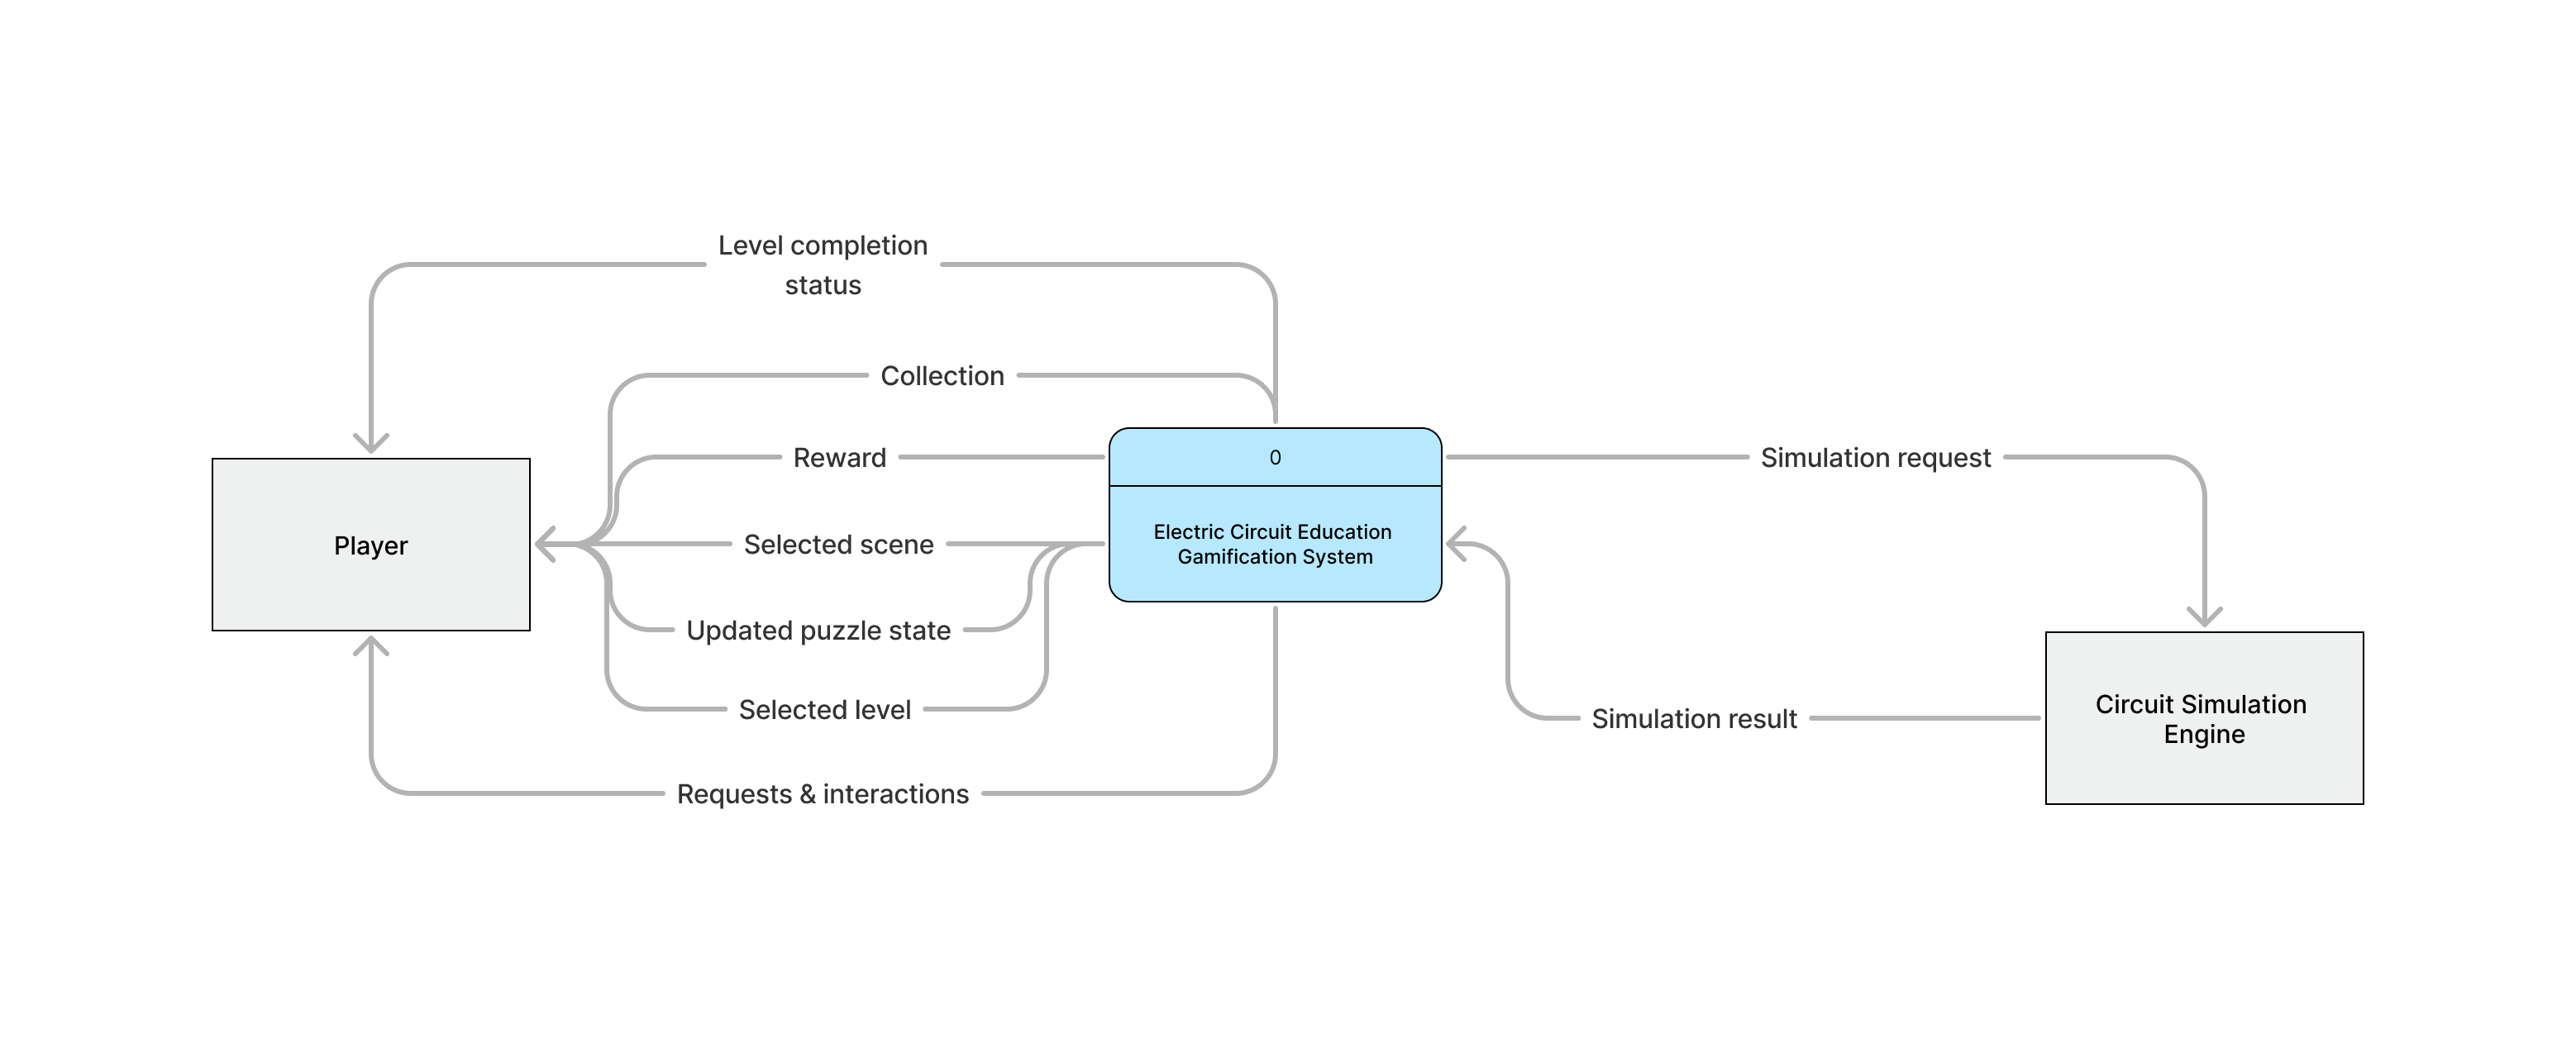
\includegraphics[scale=0.3]{images/chapter3/Context.png}
\caption{Context Diagram}
\label{Context.png}
\end{figure}
\newpage
\subsection{Process Diagram}
\begin{figure}[ht!]
\centering
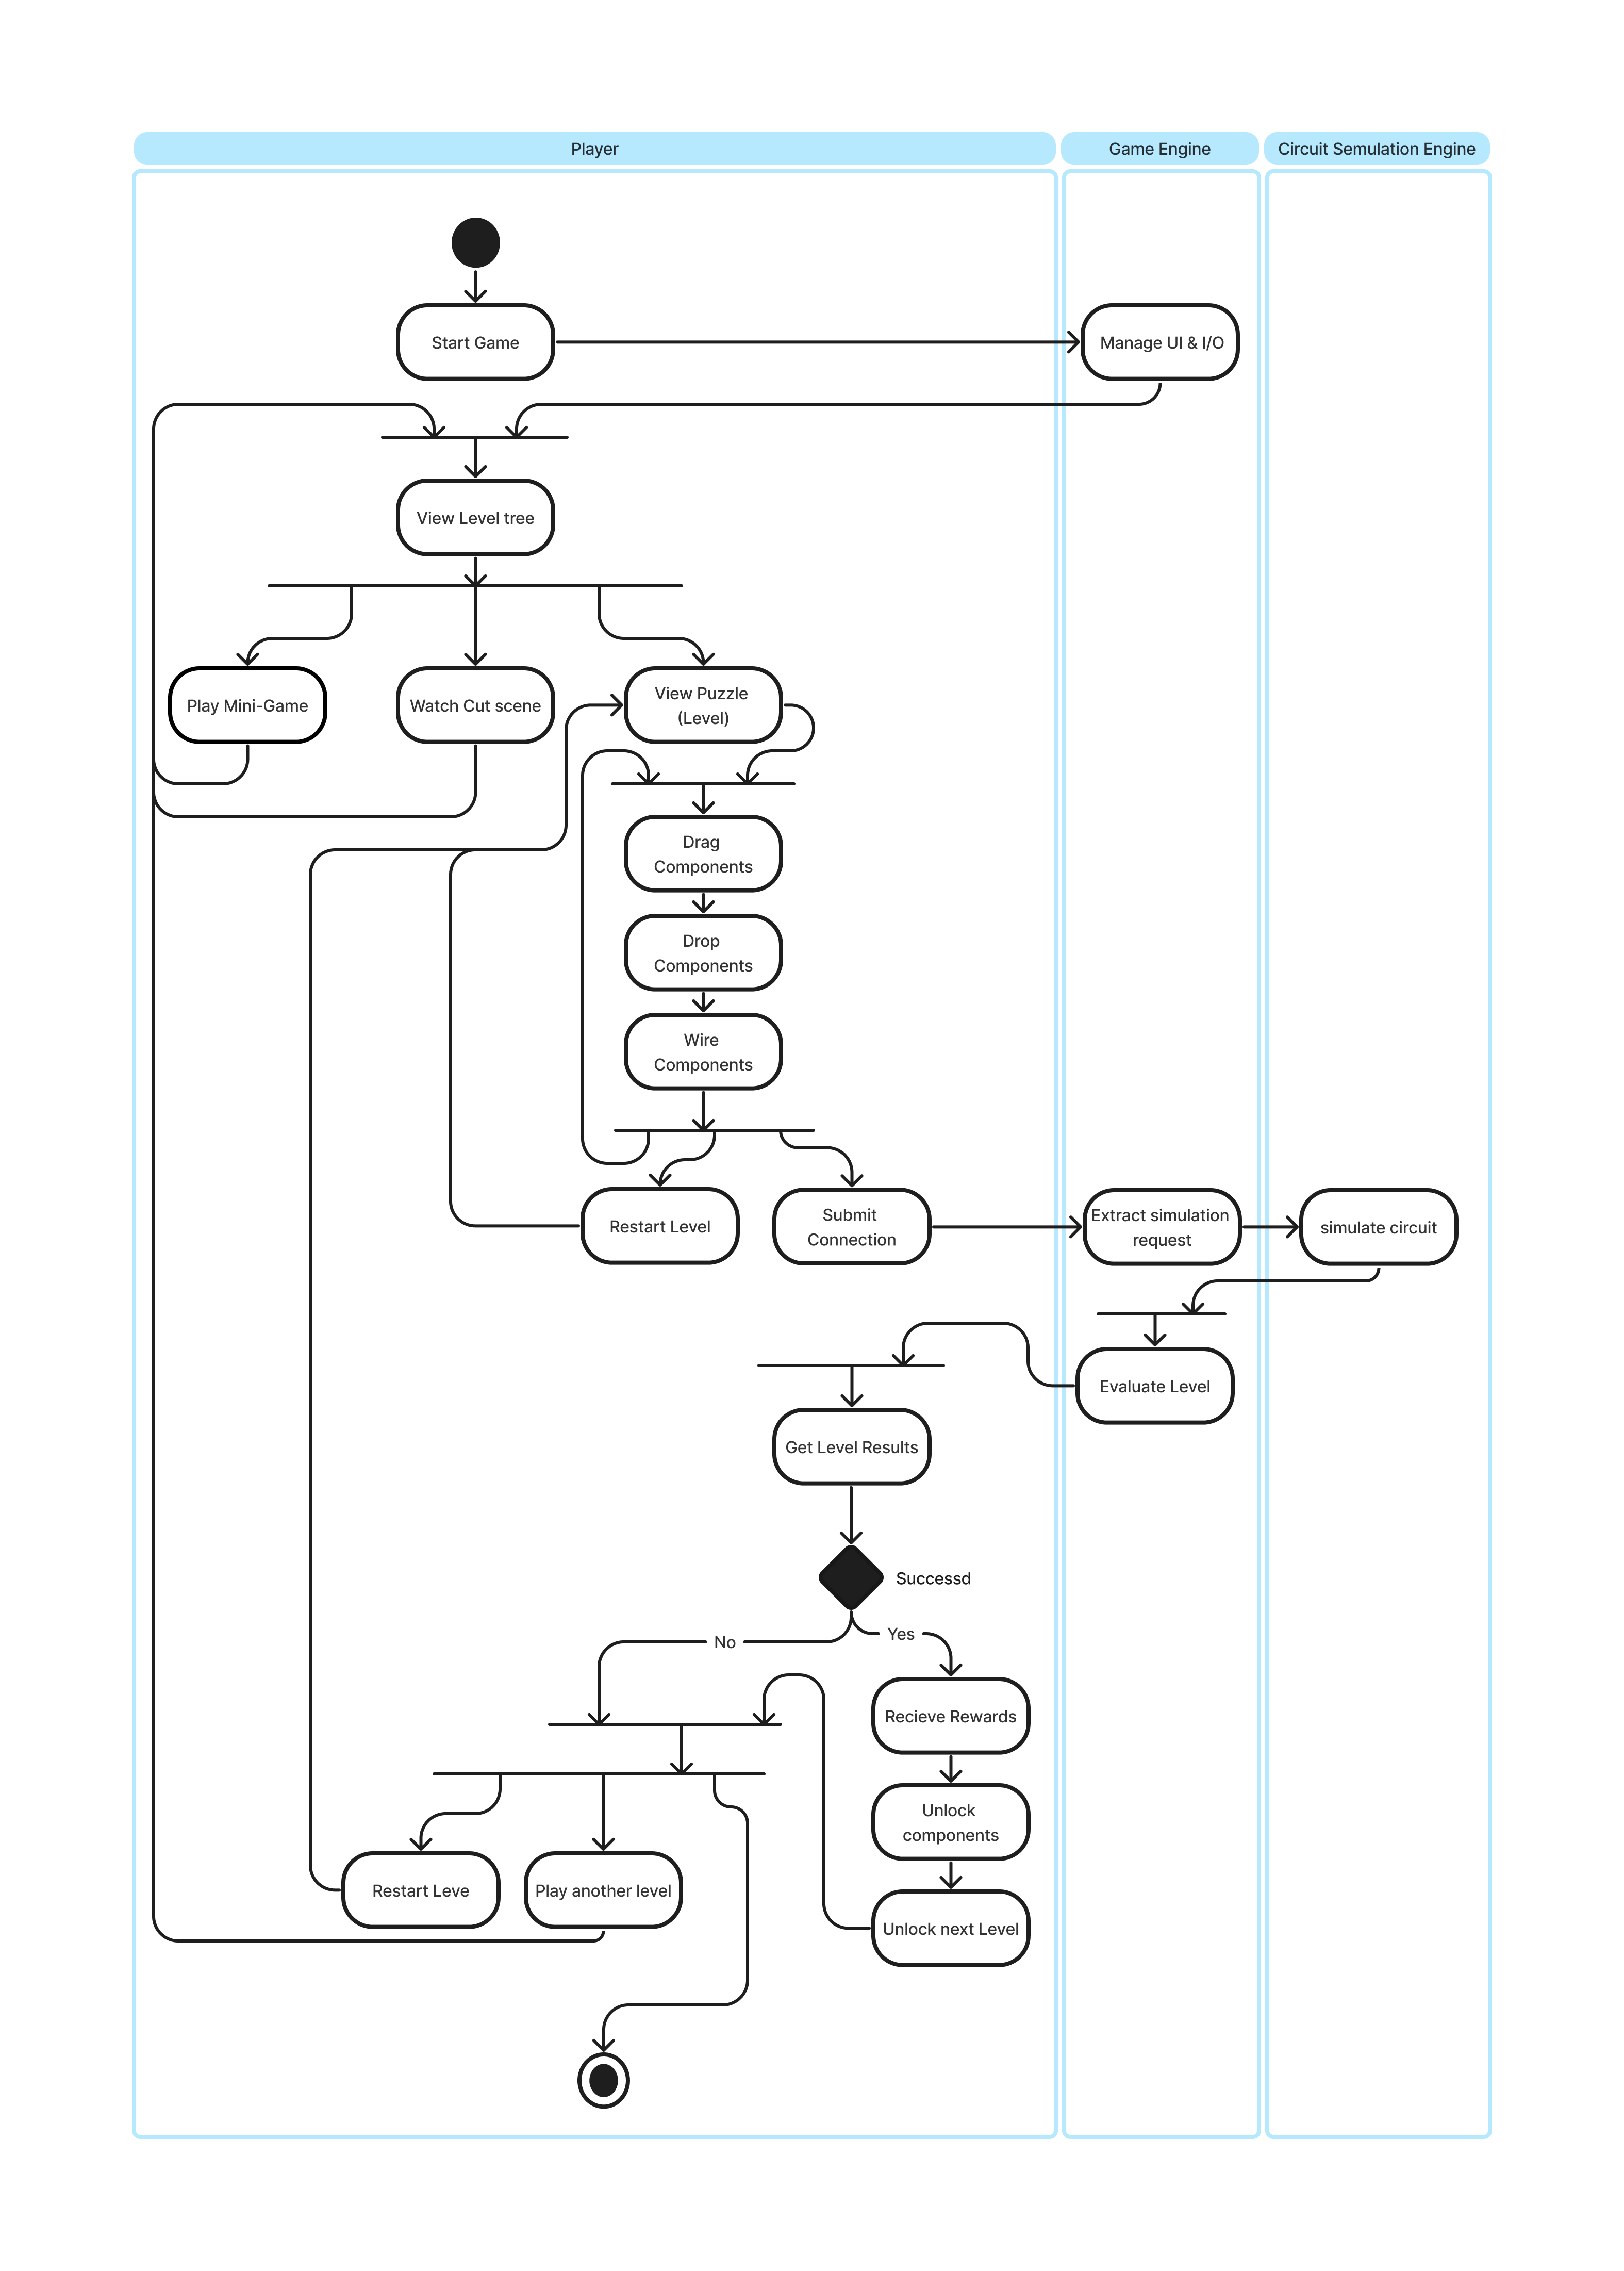
\includegraphics[scale=0.27]{images/chapter3/Process.png}
\caption{Process Diagram}
\label{prcess.png}
\end{figure}
\vfill
\newpage
\vfill
\subsection{Use Case Diagram}
\vfill
\begin{figure}[!ht]
\centering
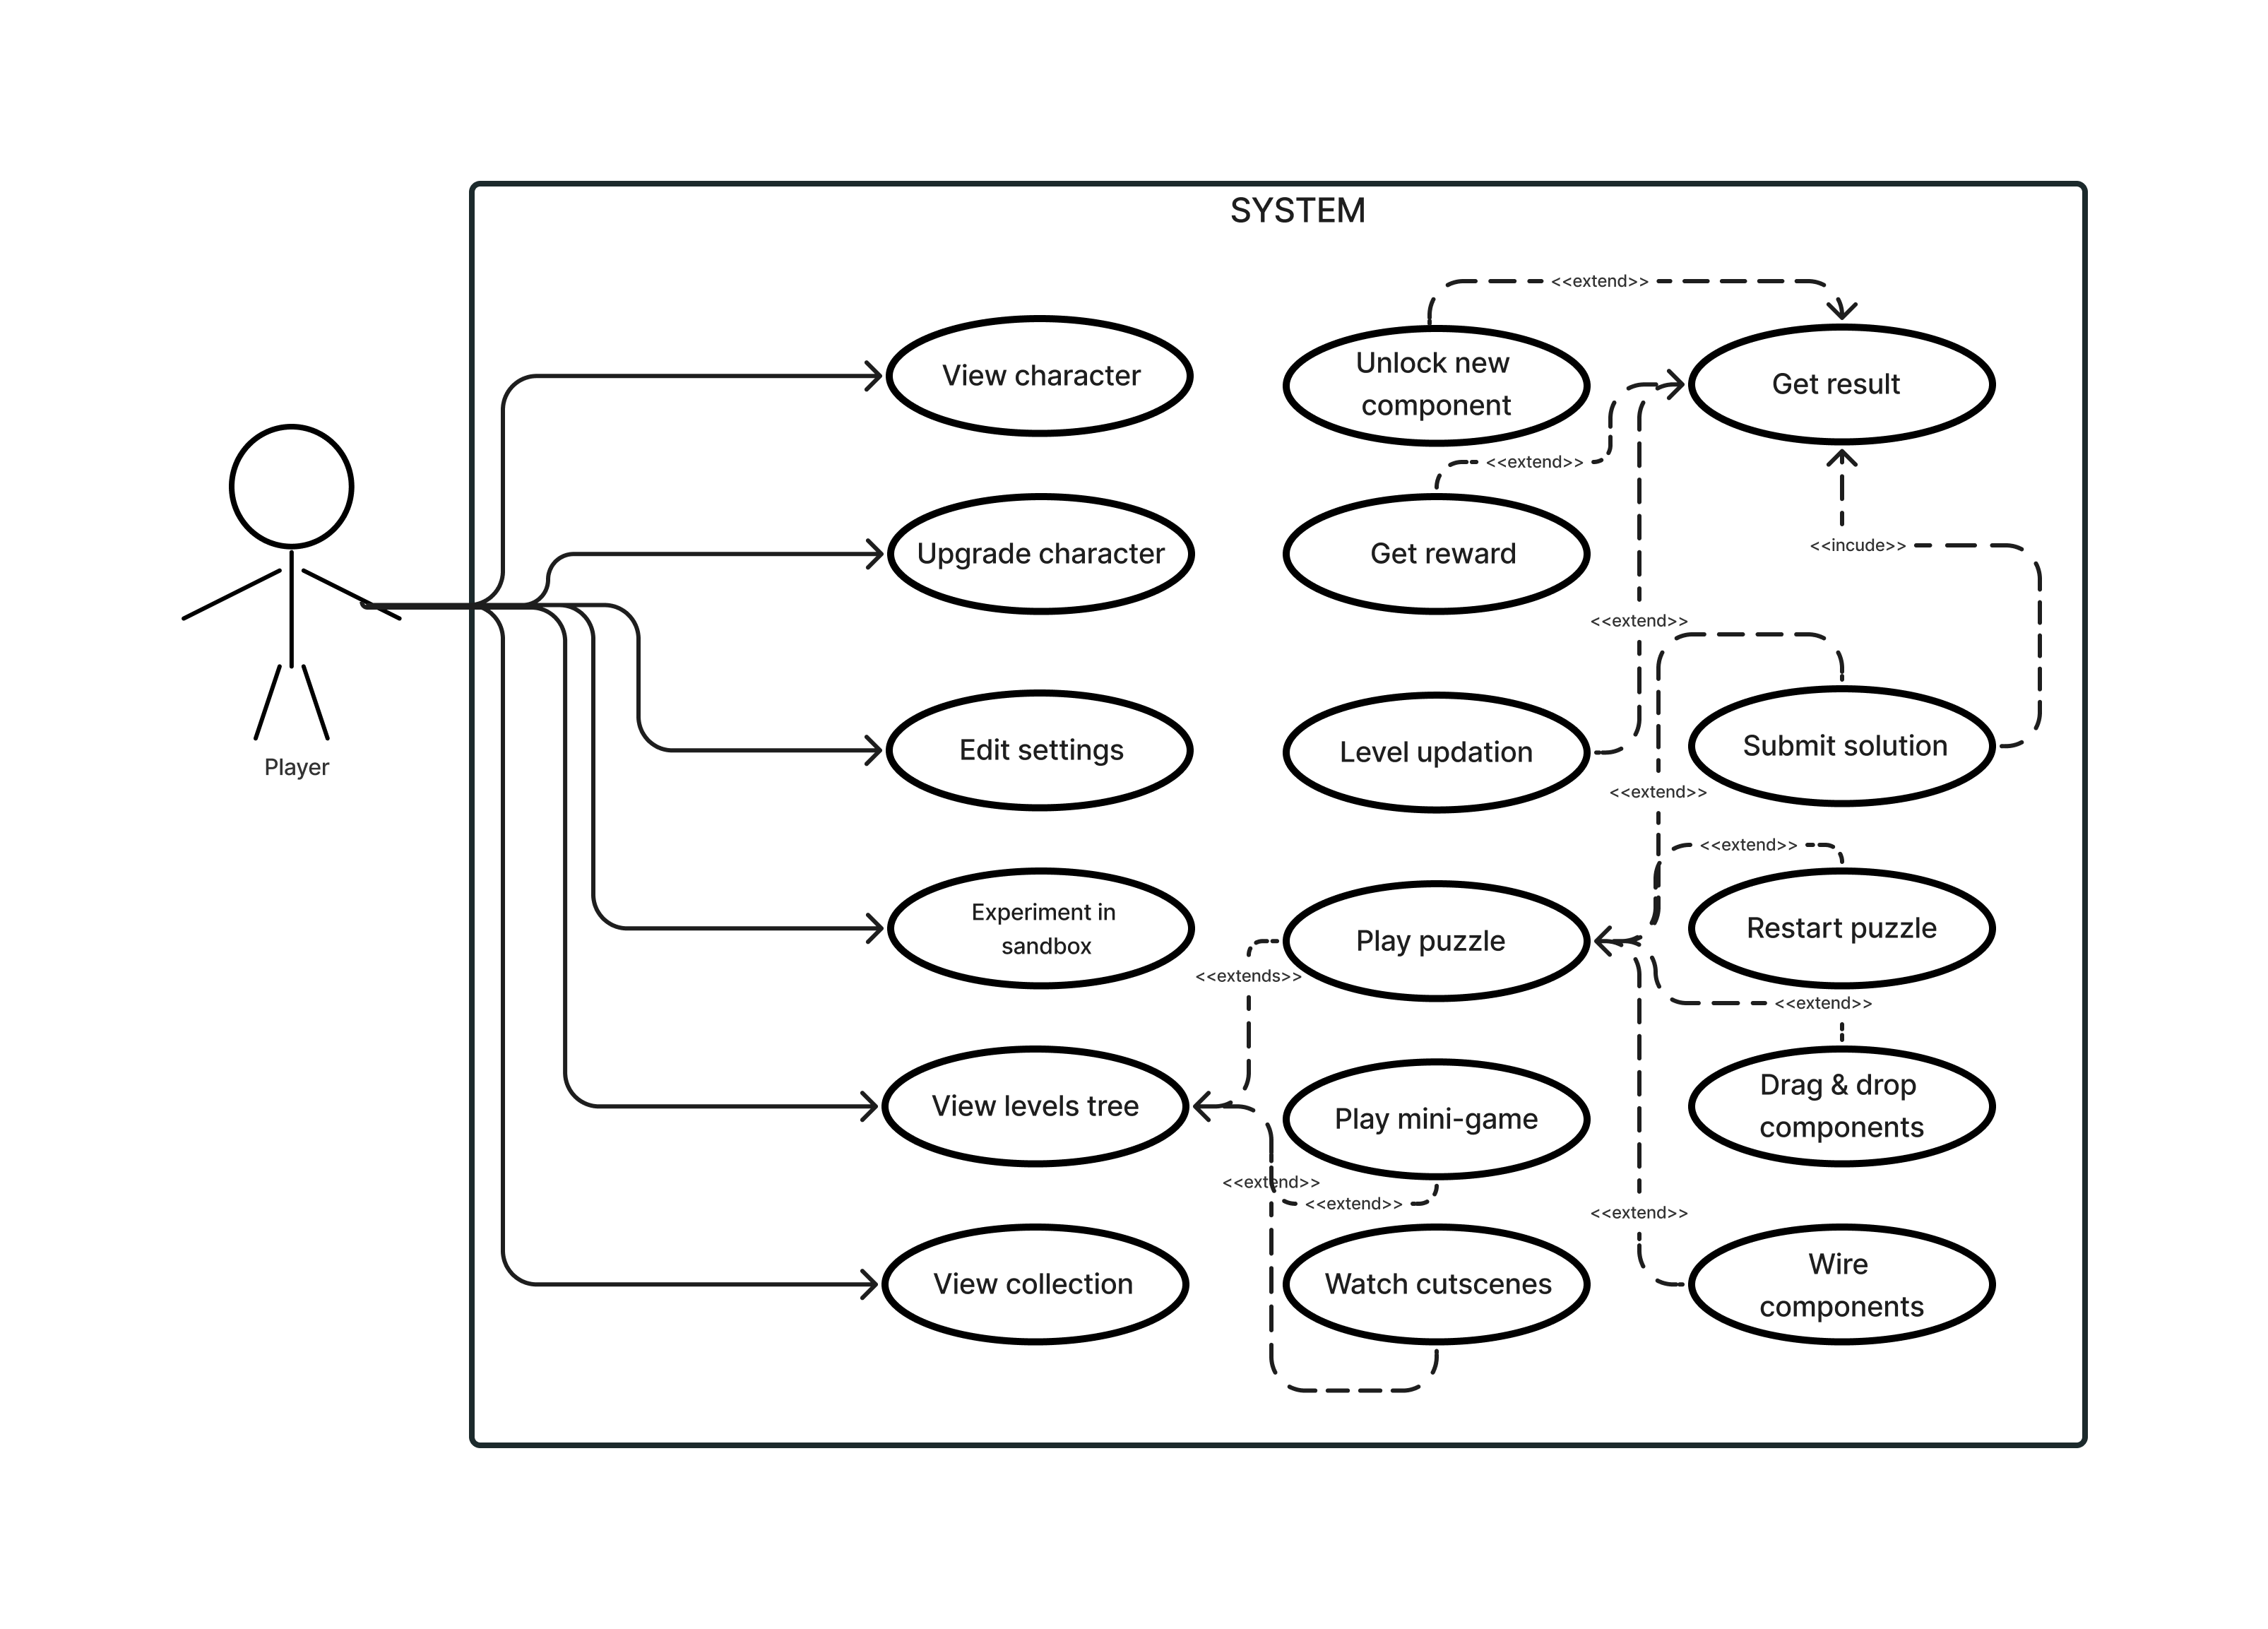
\includegraphics[scale=0.27]{images/chapter3/Usecase.png}
\caption{Usecase Diagram}
\label{Use Case.png}
\end{figure}
\vfill
\newpage
\subsection{Data-Flow Diagram}
\begin{figure}[ht!]
\centering
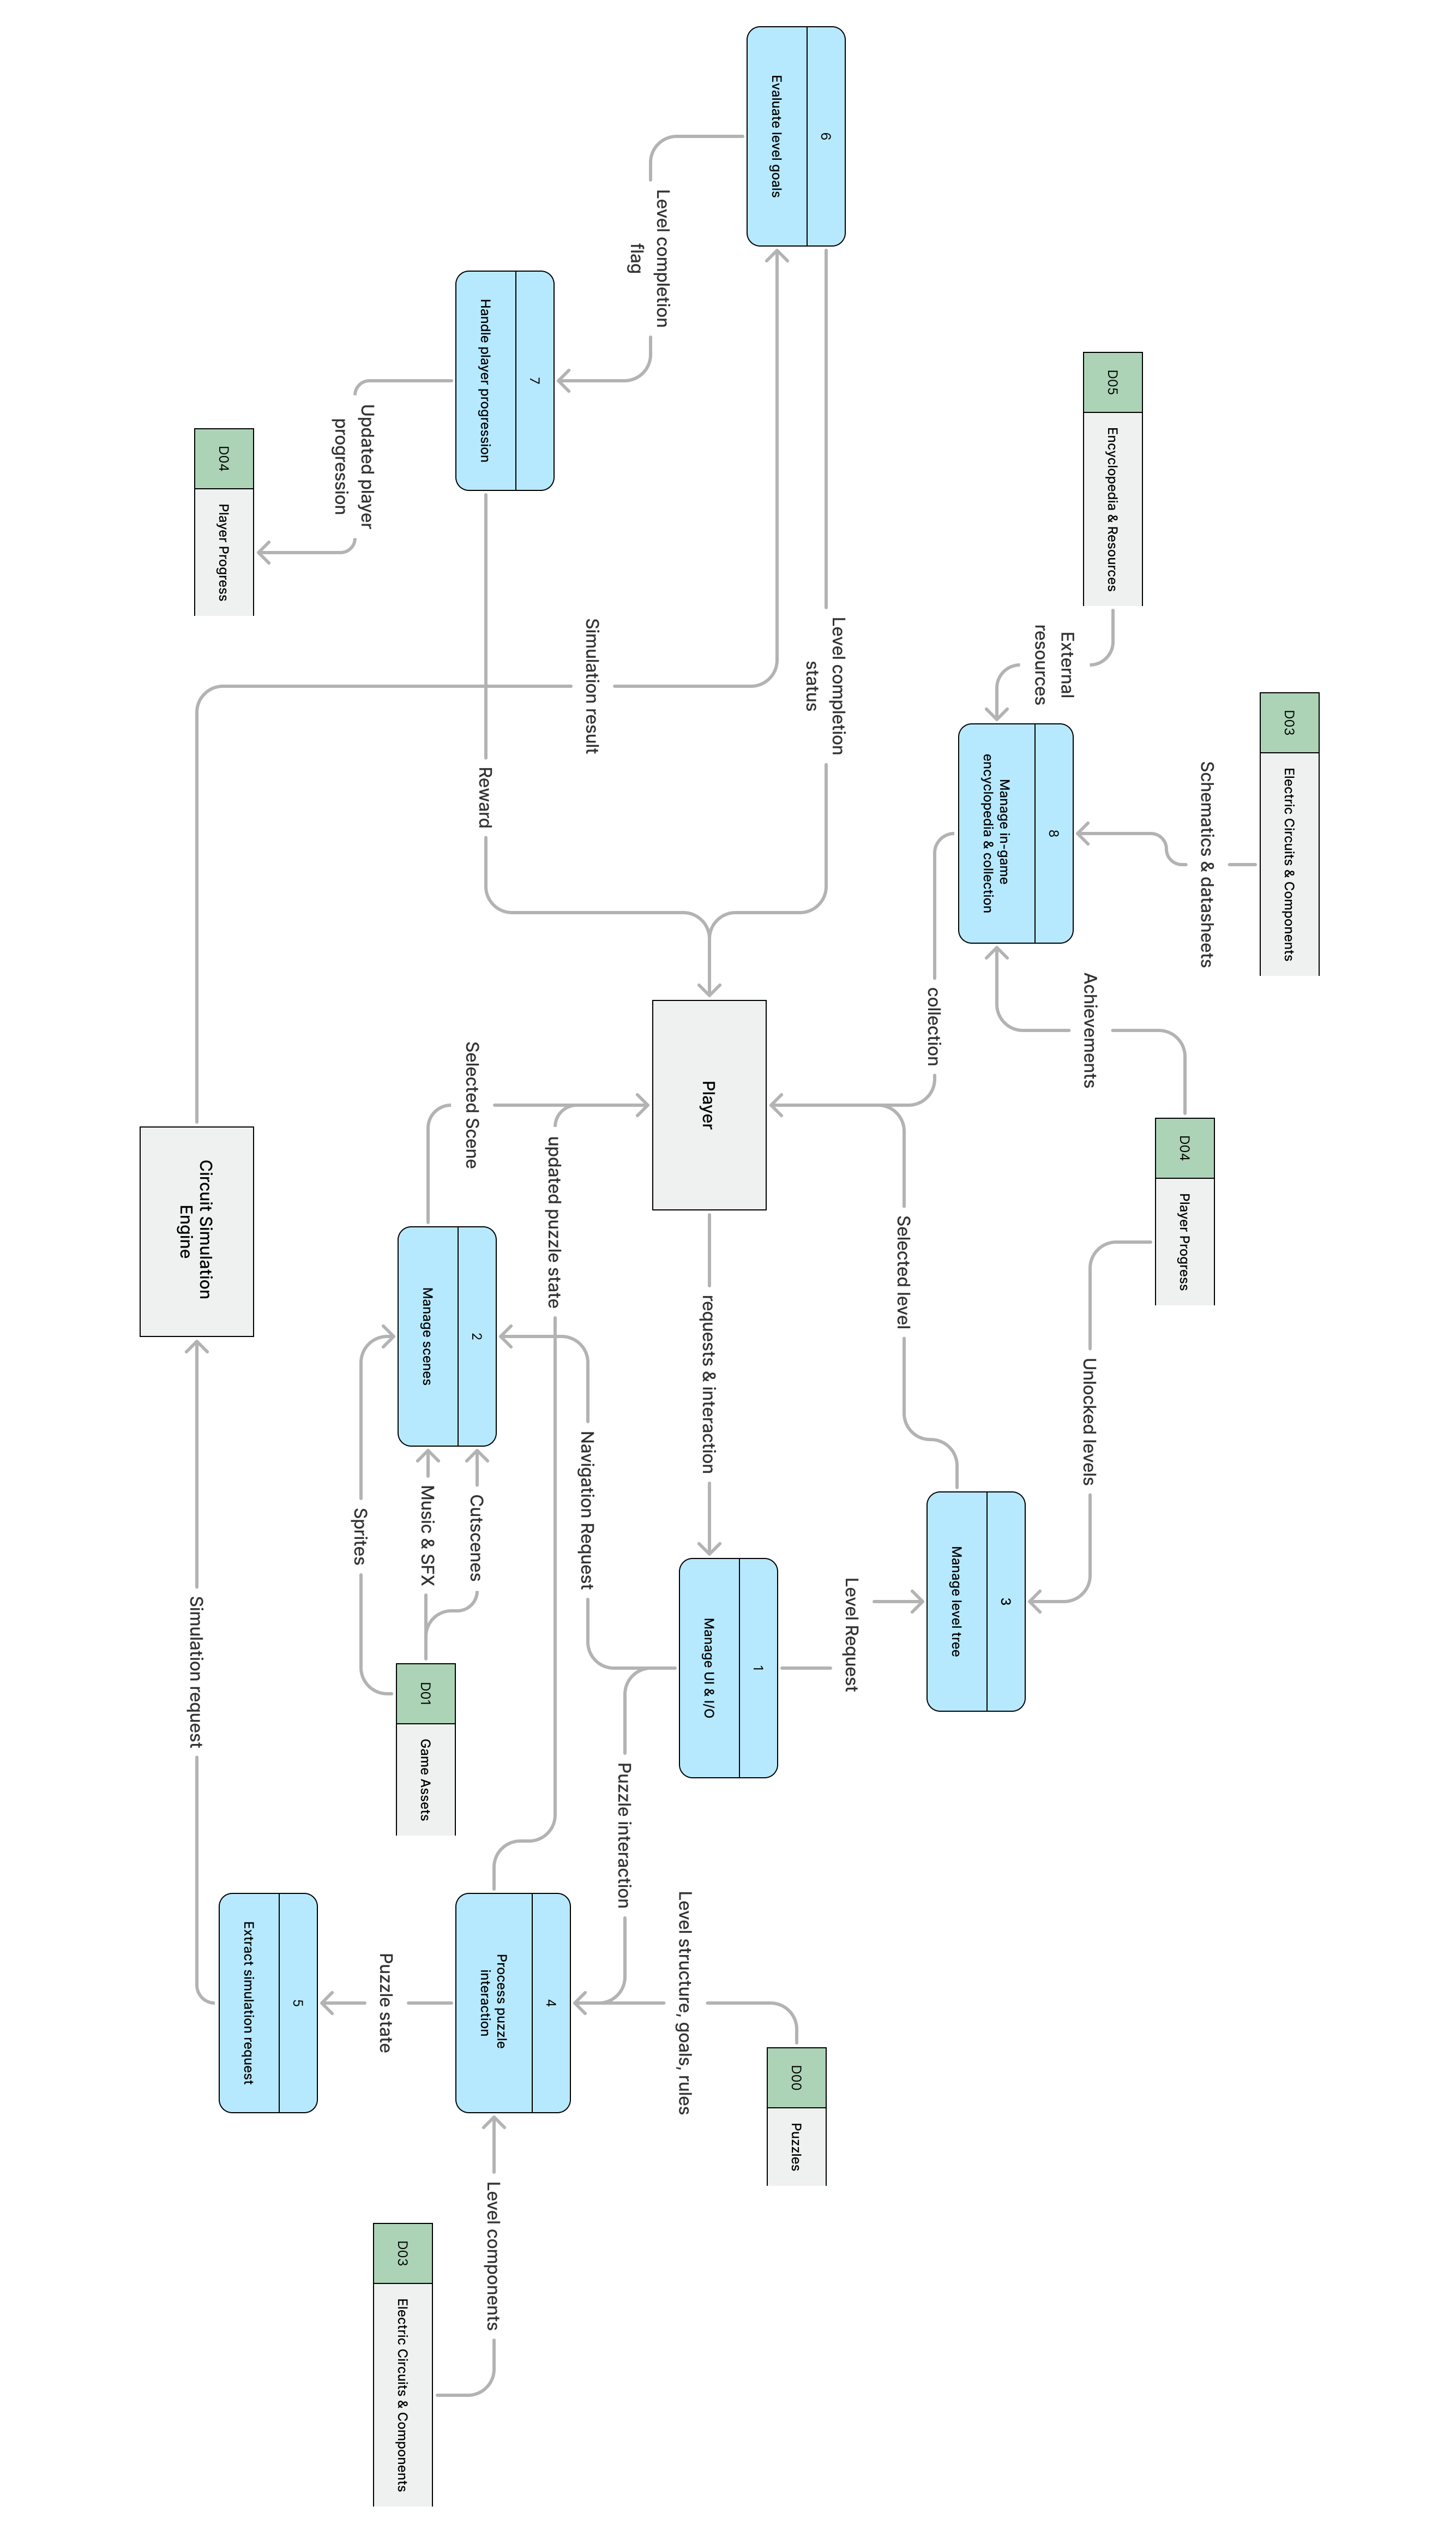
\includegraphics[scale=0.13]{images/chapter3/DFD.png}
\caption{Data-Flow Diagram}
\label{Data-Flow Diagram}
\end{figure}
\vfill
\newpage
\subsection{Sequence Diagram}
\begin{figure}[h!t]
\centering
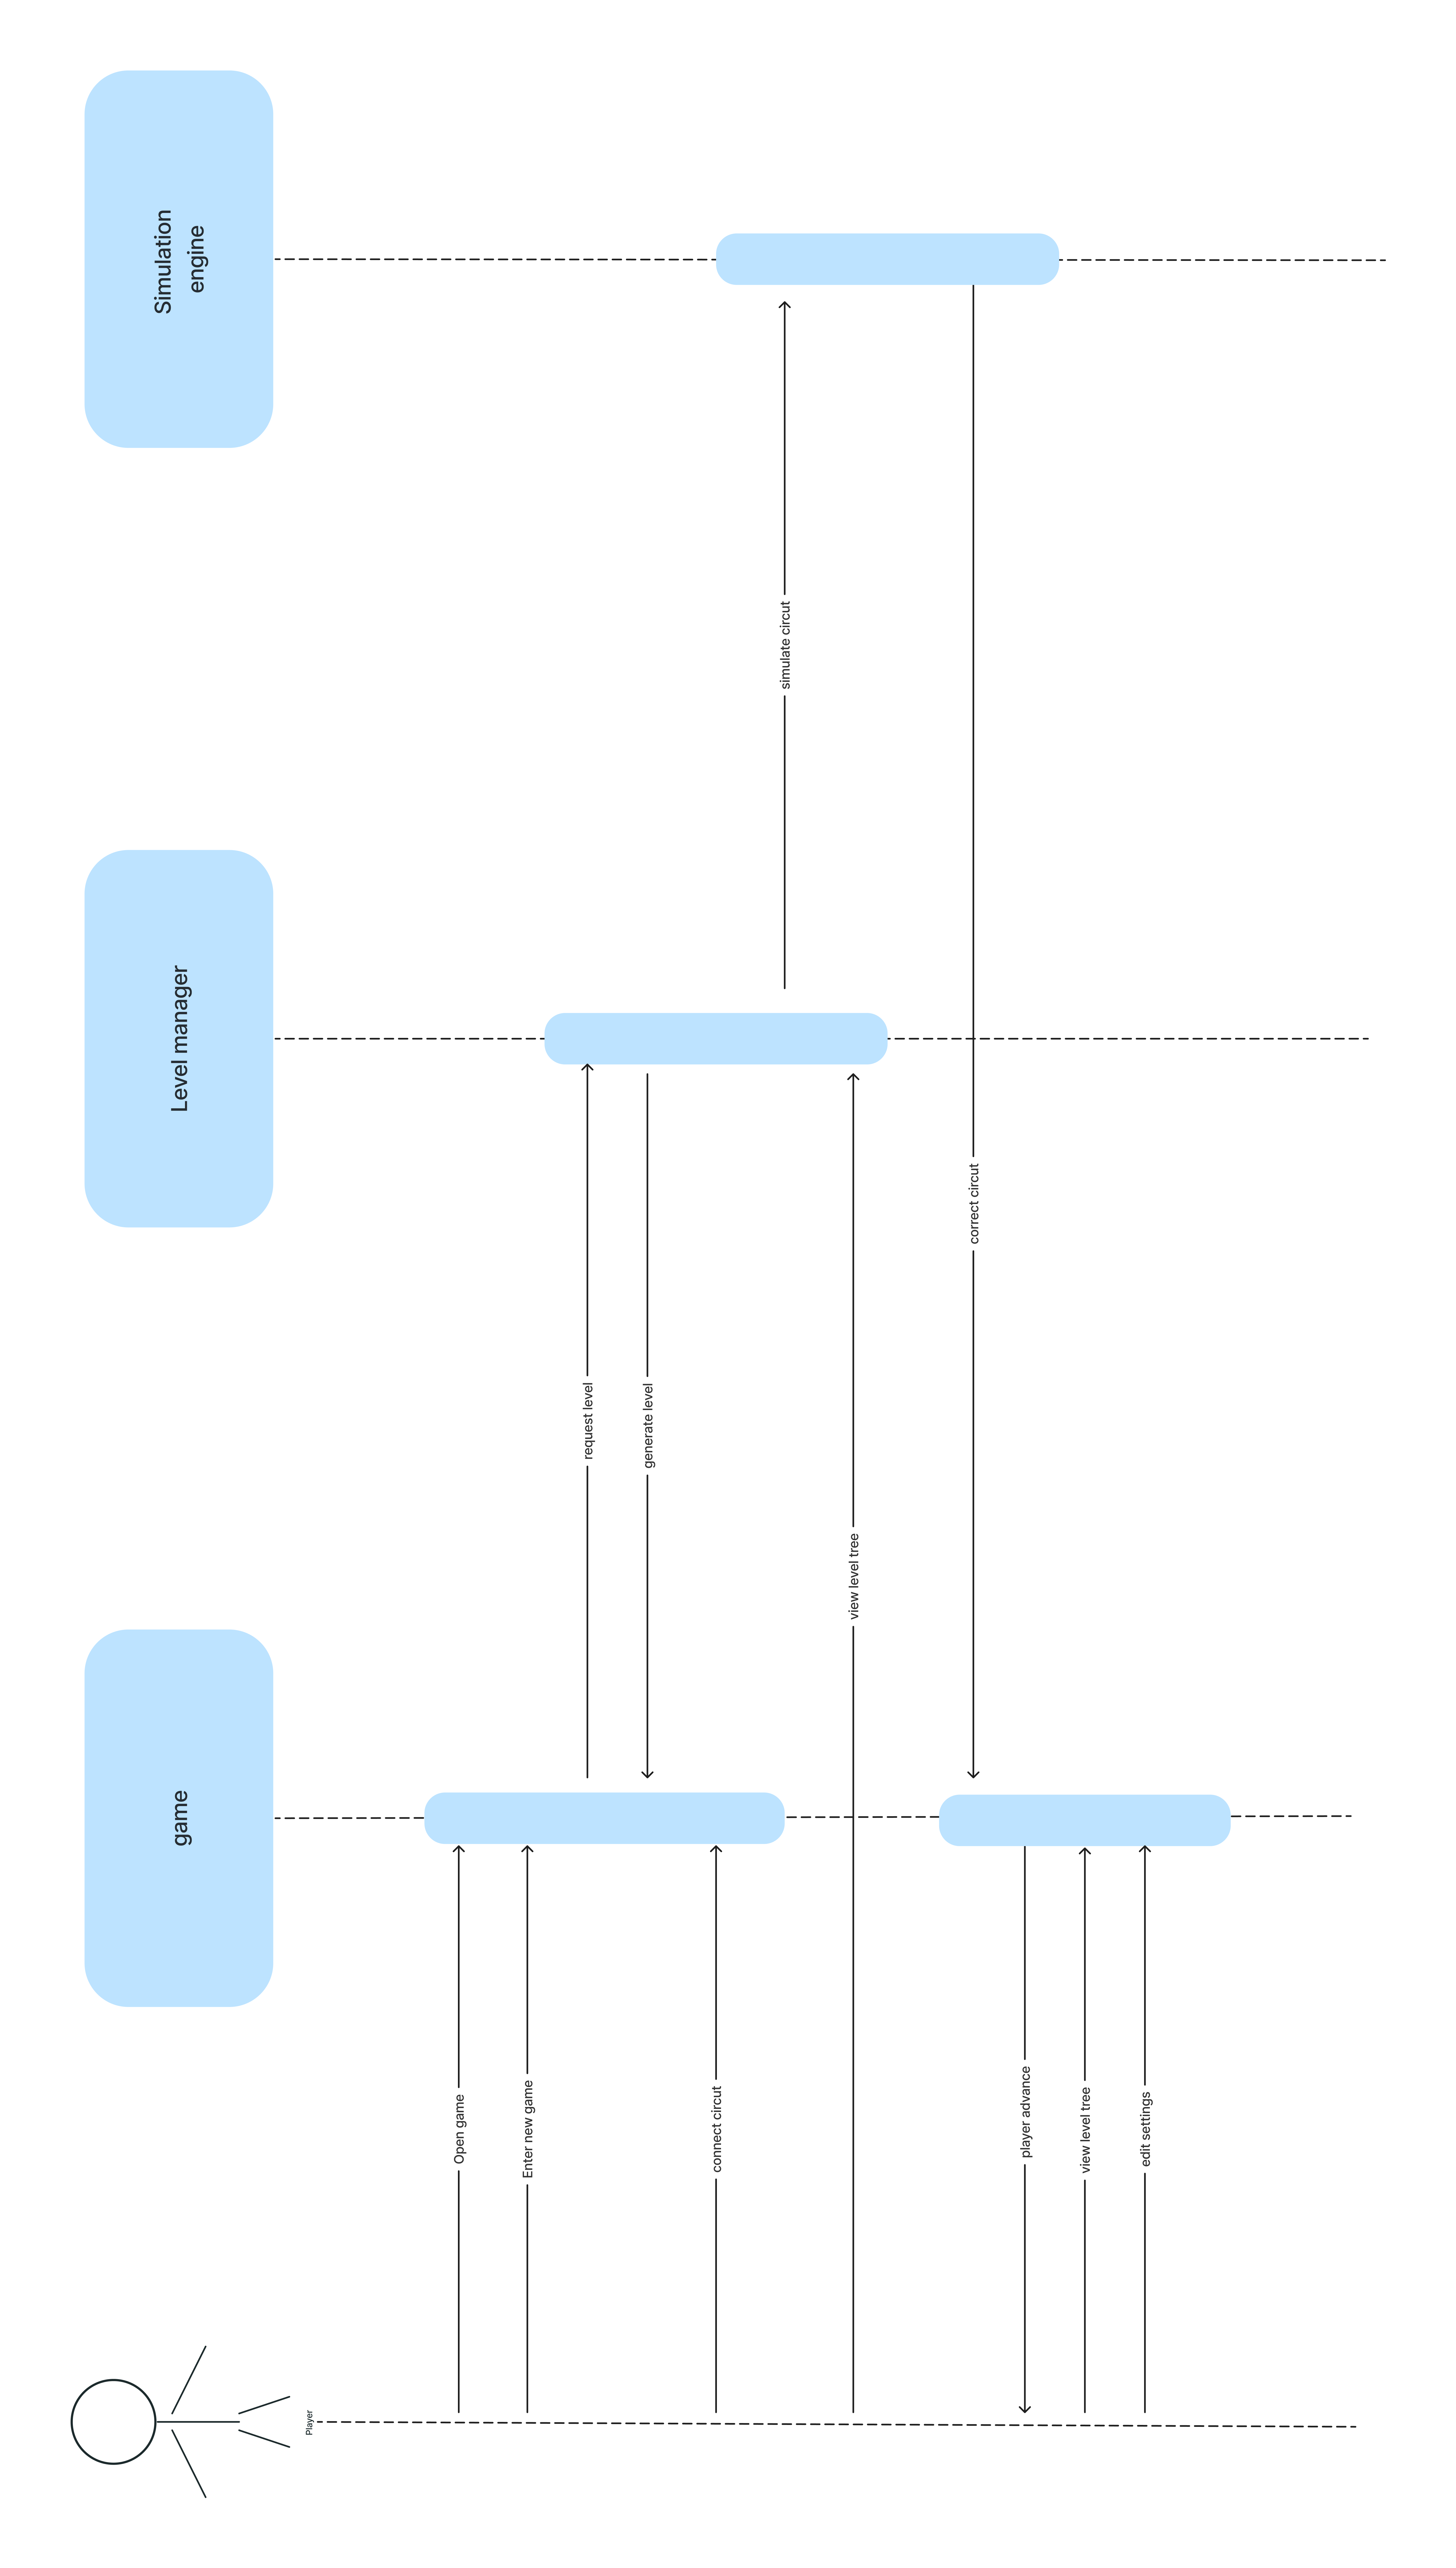
\includegraphics[scale=0.11]{images/chapter3/sq.png}
\caption{Sequence Diagram}
\label{Sequence Diagram}
\end{figure}
\vfill
\newpage
\subsection{Class Diagram}

\subsubsection{Simulator and Simulation Manager}

\begin{figure}[h!t]
\centering
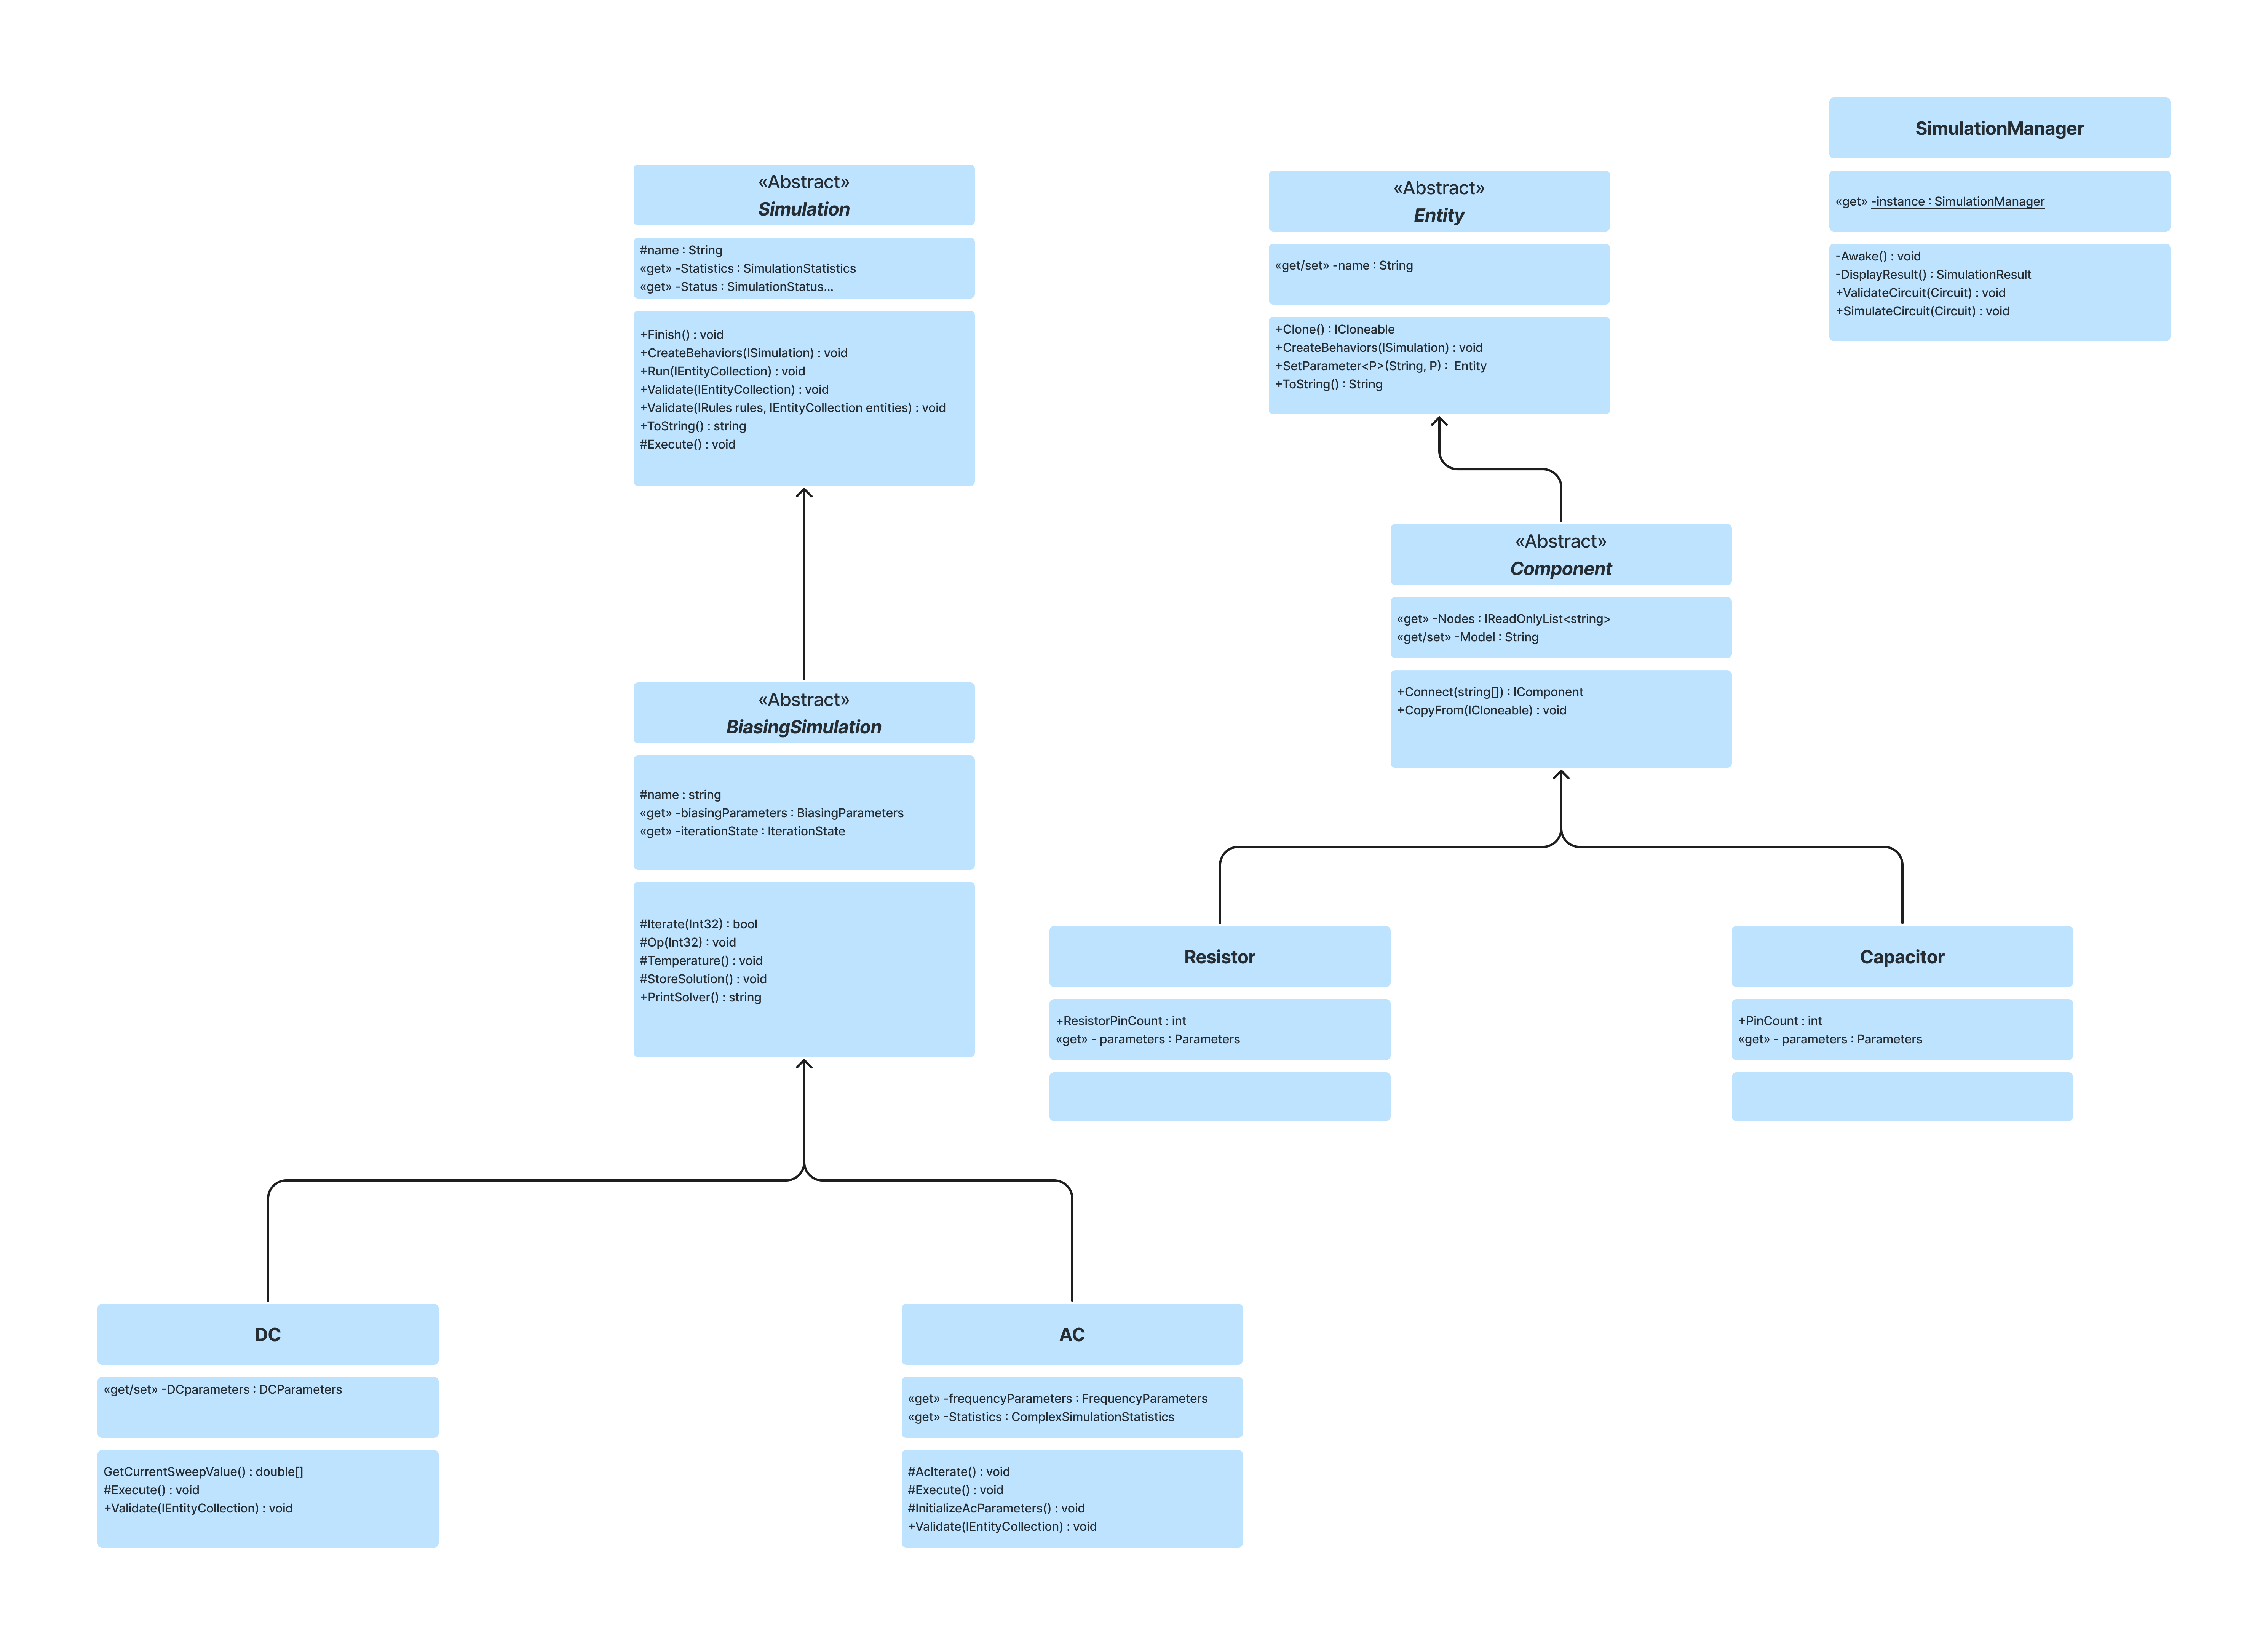
\includegraphics[scale=0.12]{images/chapter3/Class1.png}
\caption{Simulator and Simulation Manager Class Diagram}
\label{Simulator and Simulation Manager}
\end{figure}

\subsubsection{GameComponents and ComponentManager}

\begin{figure}[h!t]
\centering
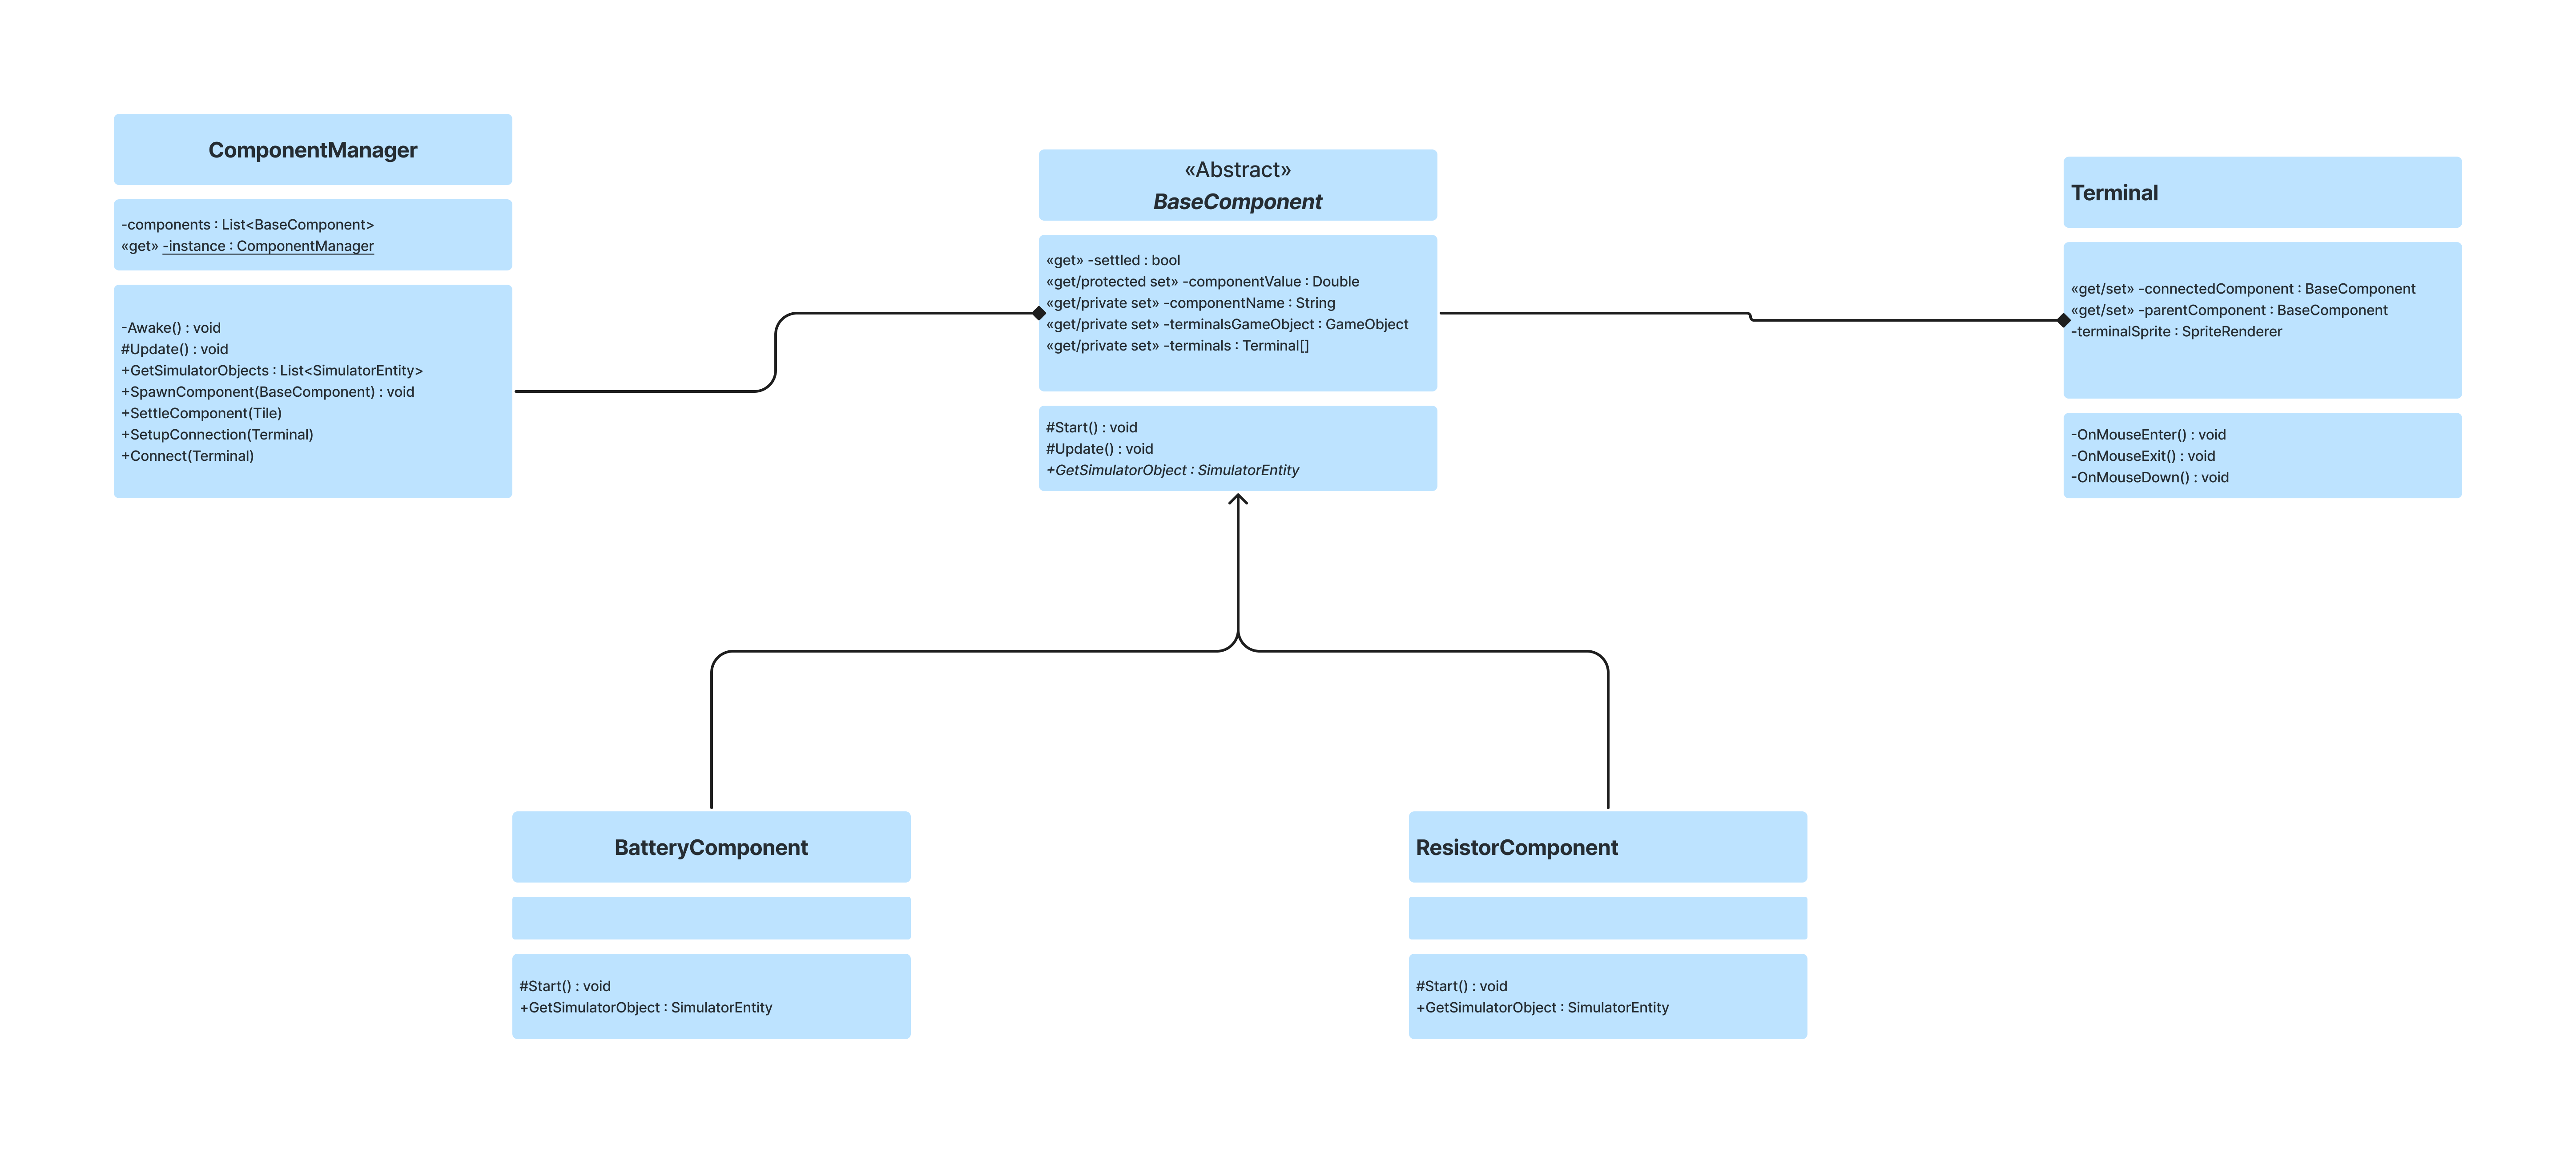
\includegraphics[scale=0.12]{images/chapter3/Class2.png}
\caption{GameComponents and ComponentManager Class Diagram}
\label{GameComponents and ComponentManager }
\end{figure}
\newpage
\subsubsection{GameManager}\begin{figure}[h!]
\centering
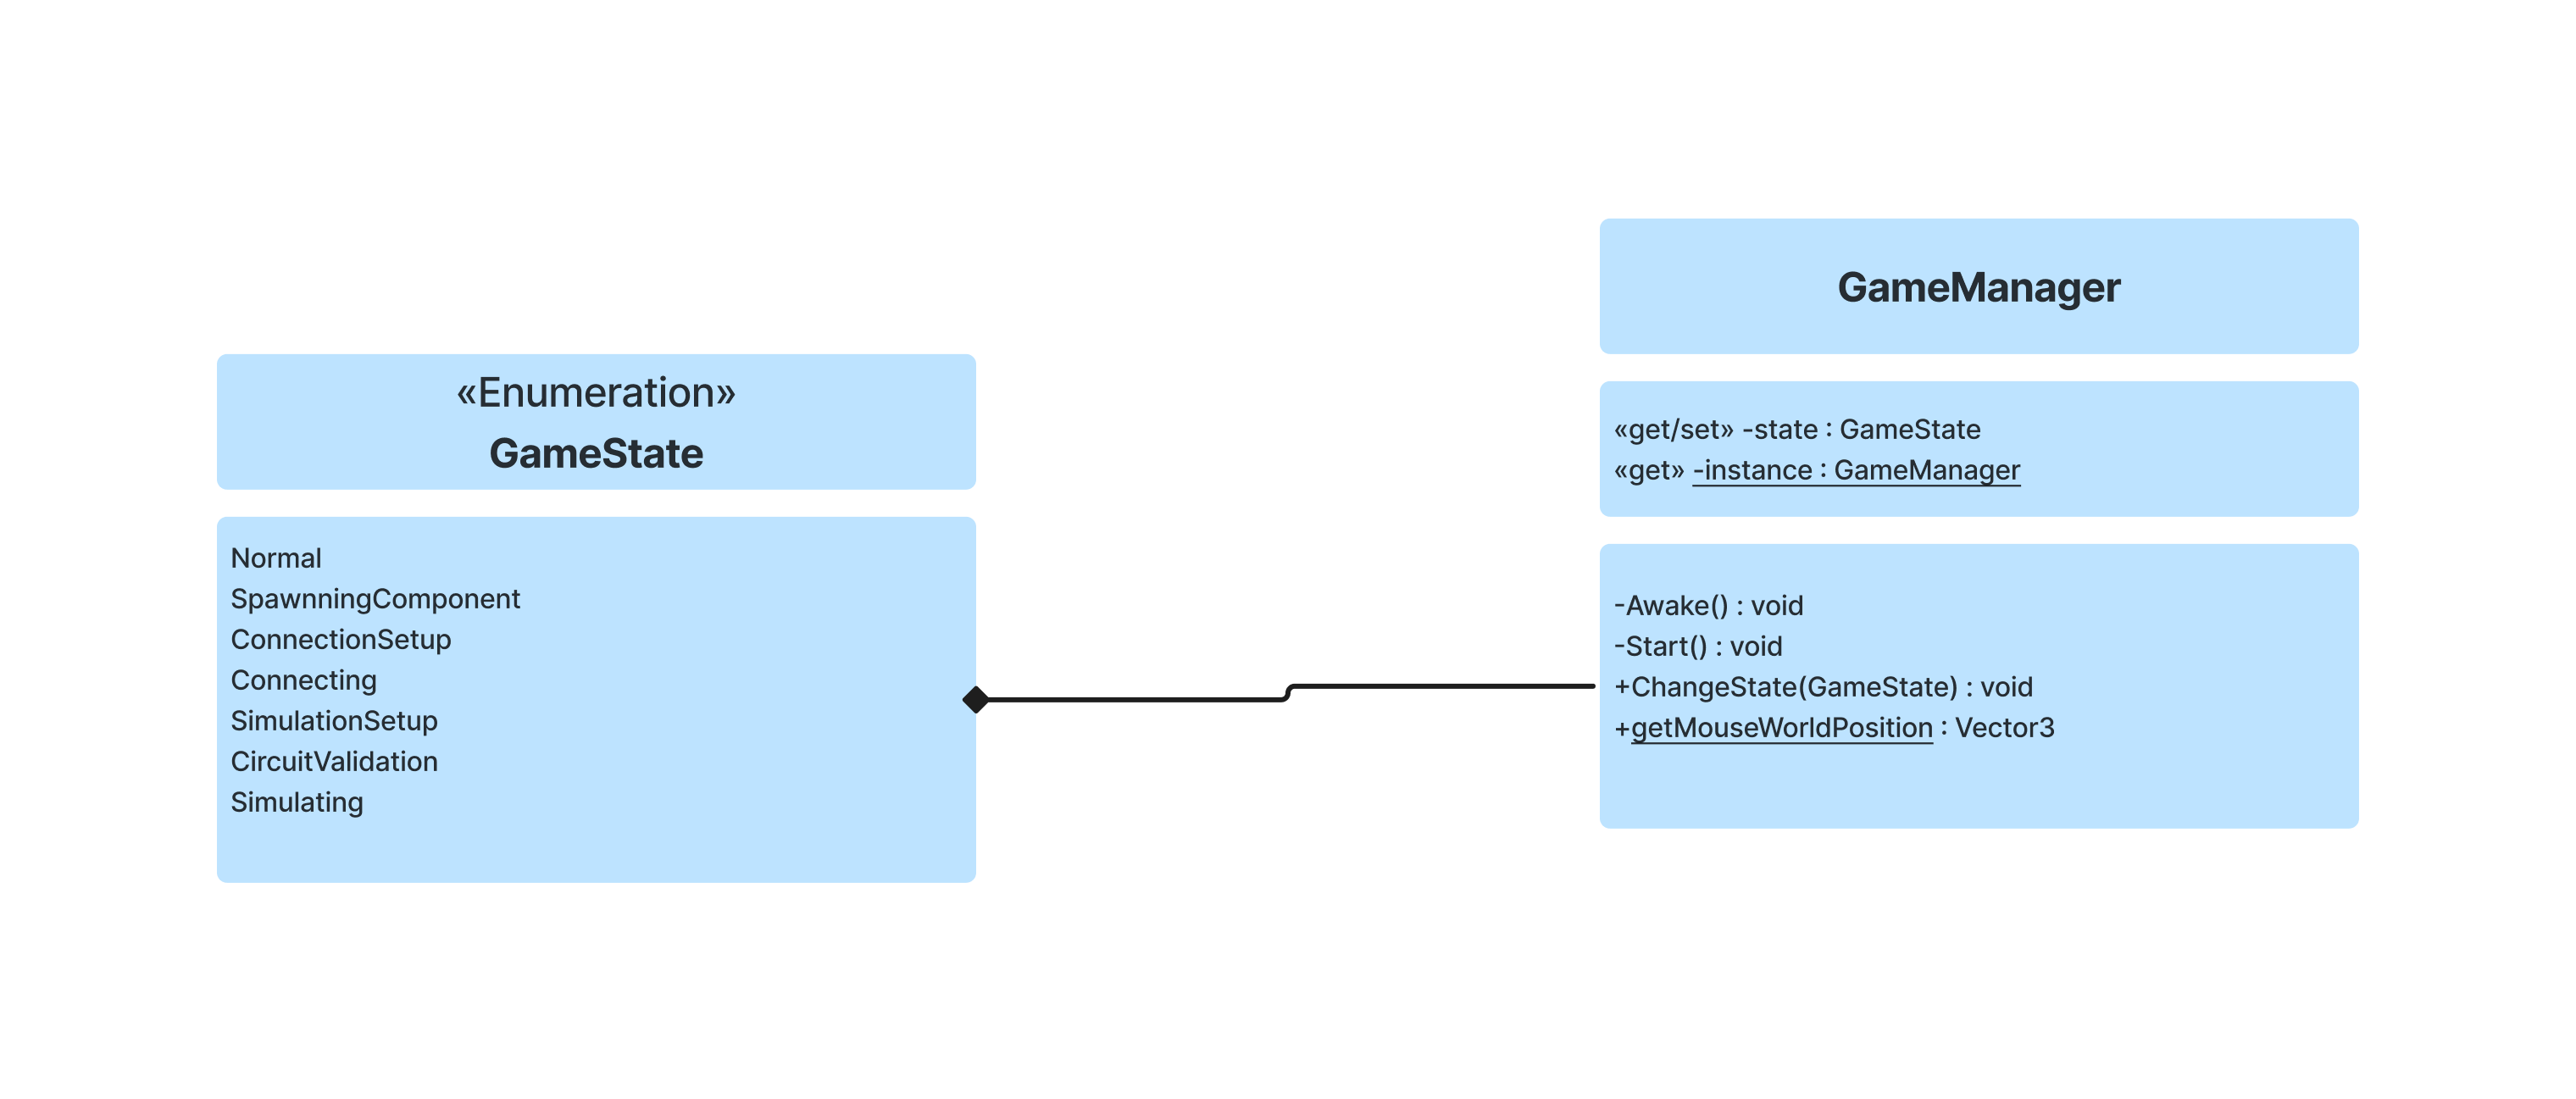
\includegraphics[scale=0.2]{images/chapter3/Class3.png}
\caption{GameManager Class Diagram}
\label{GameManager }
\end{figure}
\vfill
\newpage
\subsection{Entity Relation Diagram }
\begin{figure}[h!]
\centering
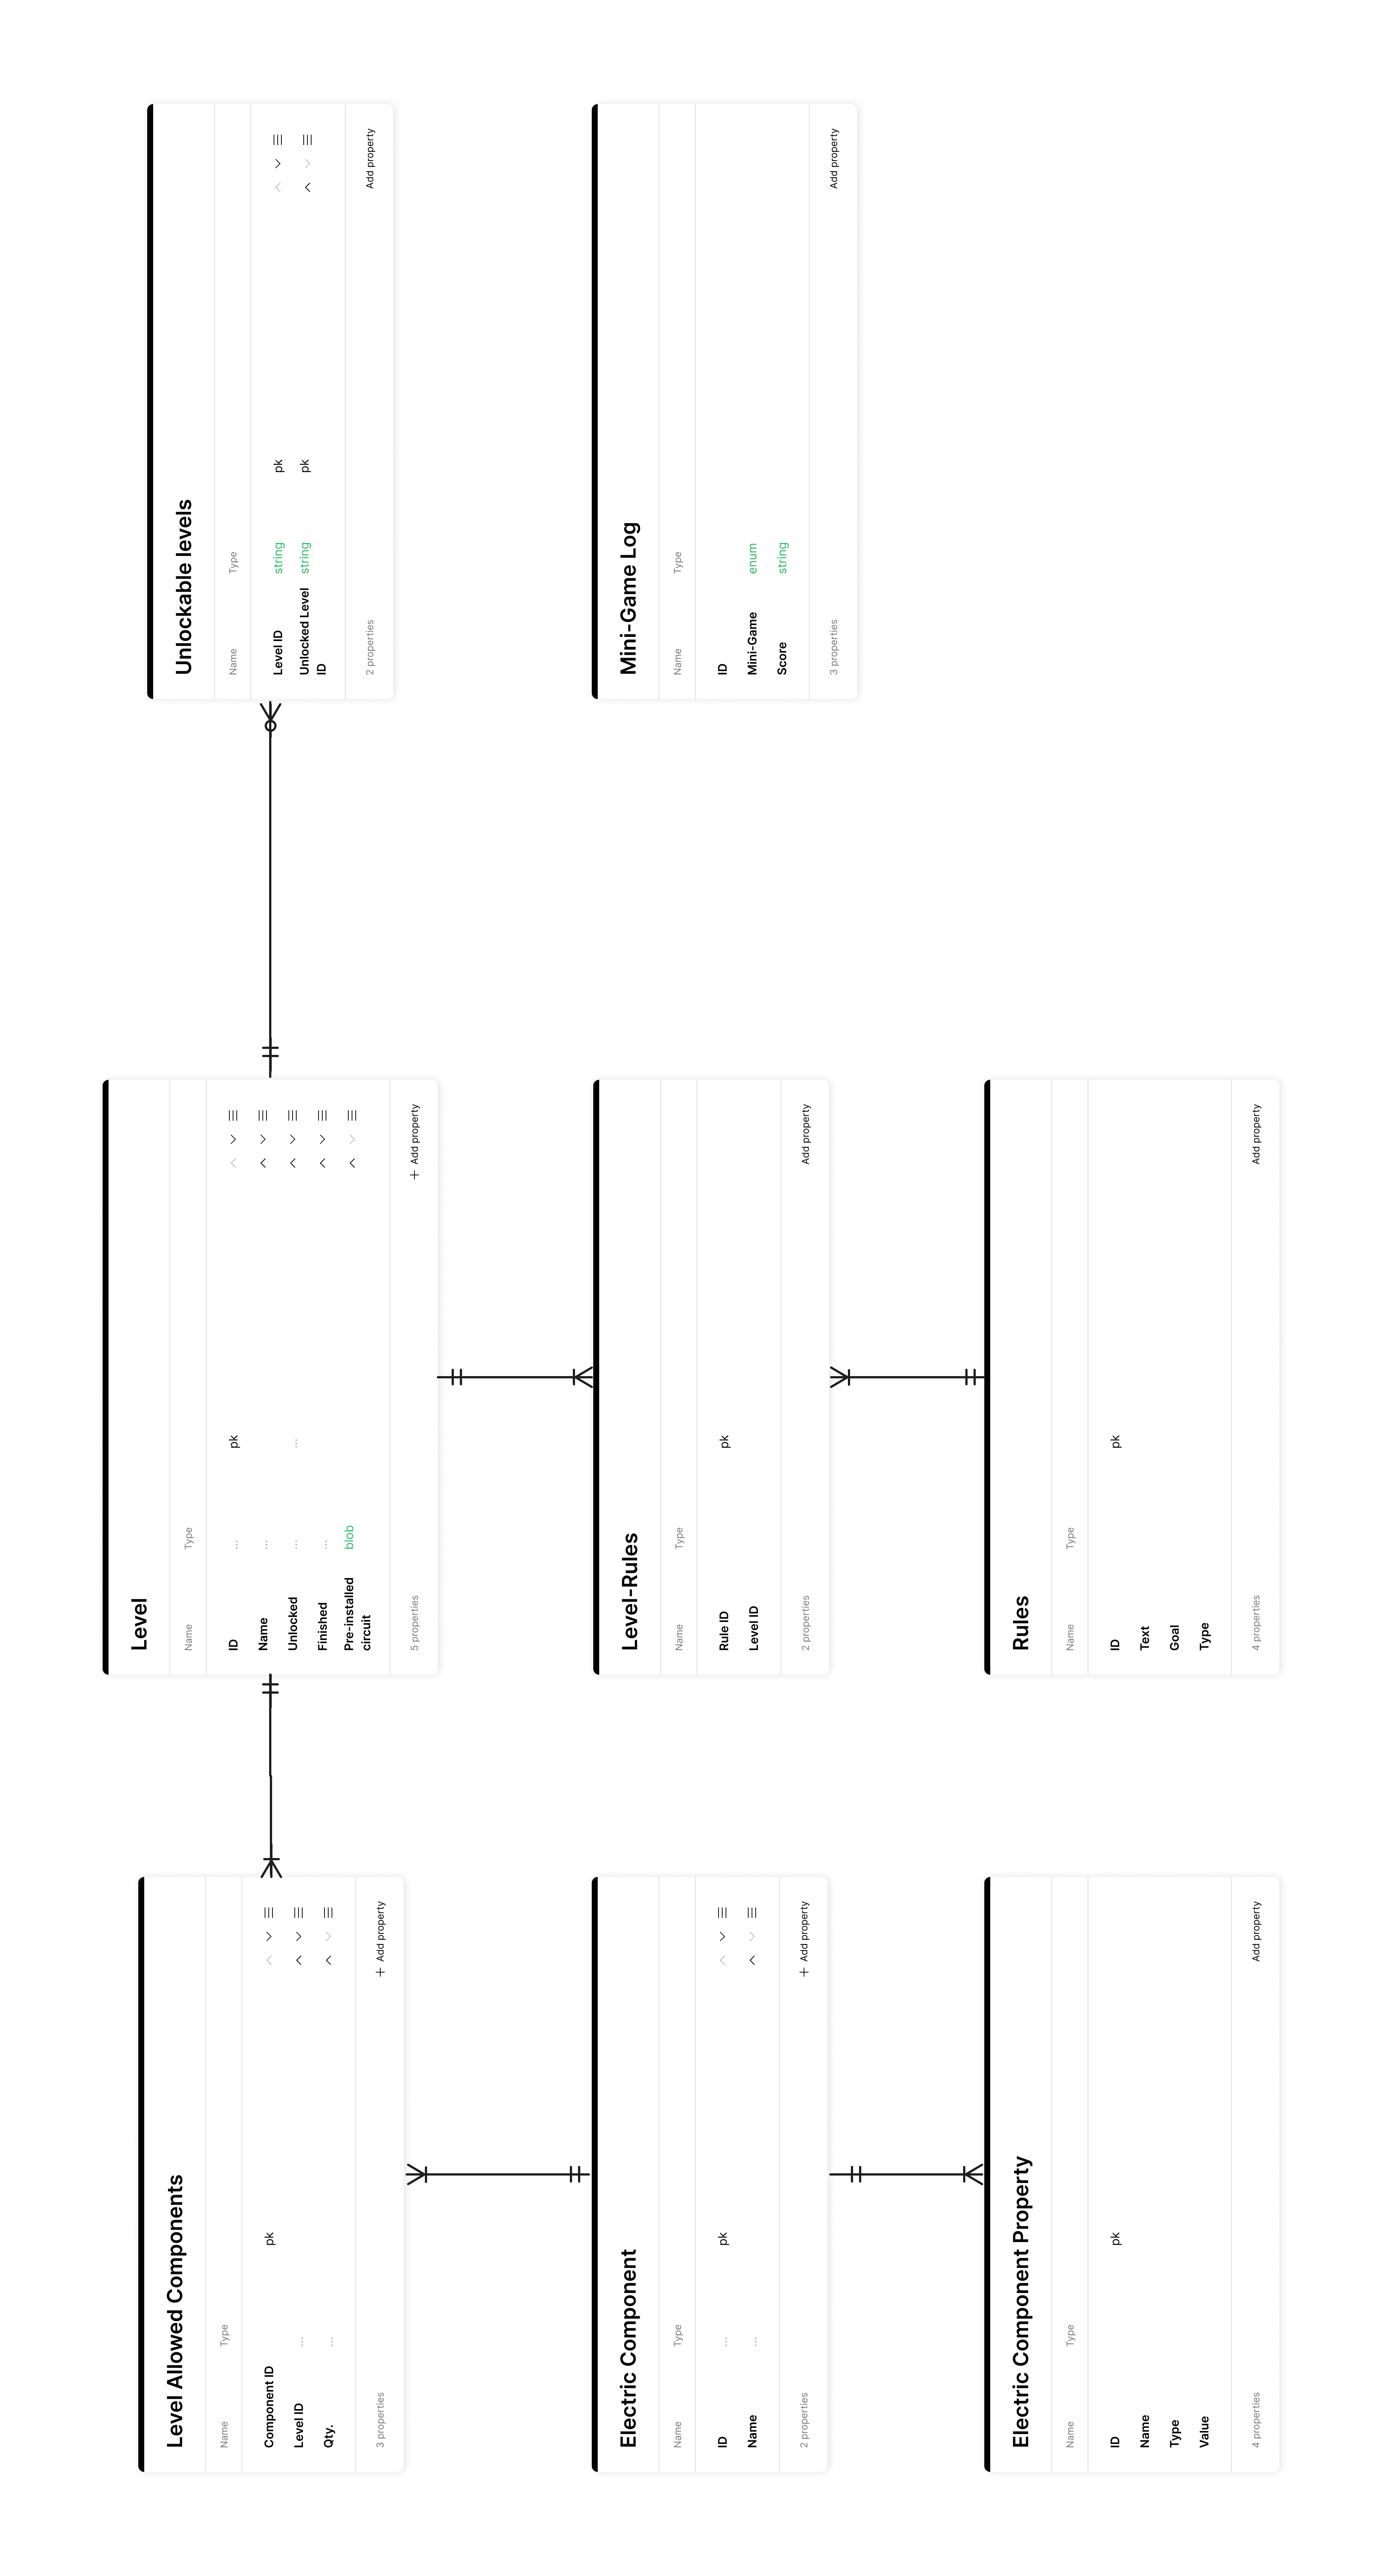
\includegraphics[scale=0.08]{images/chapter3/ERD.png}
\caption{Entity Relation Diagram }
\label{Entity Relation Diagram }
\end{figure}
\vfill
\newpage

\subsection{State Chart Diagram}
\subsubsection{Drag and drop components}

\begin{figure}[h!]
\centering
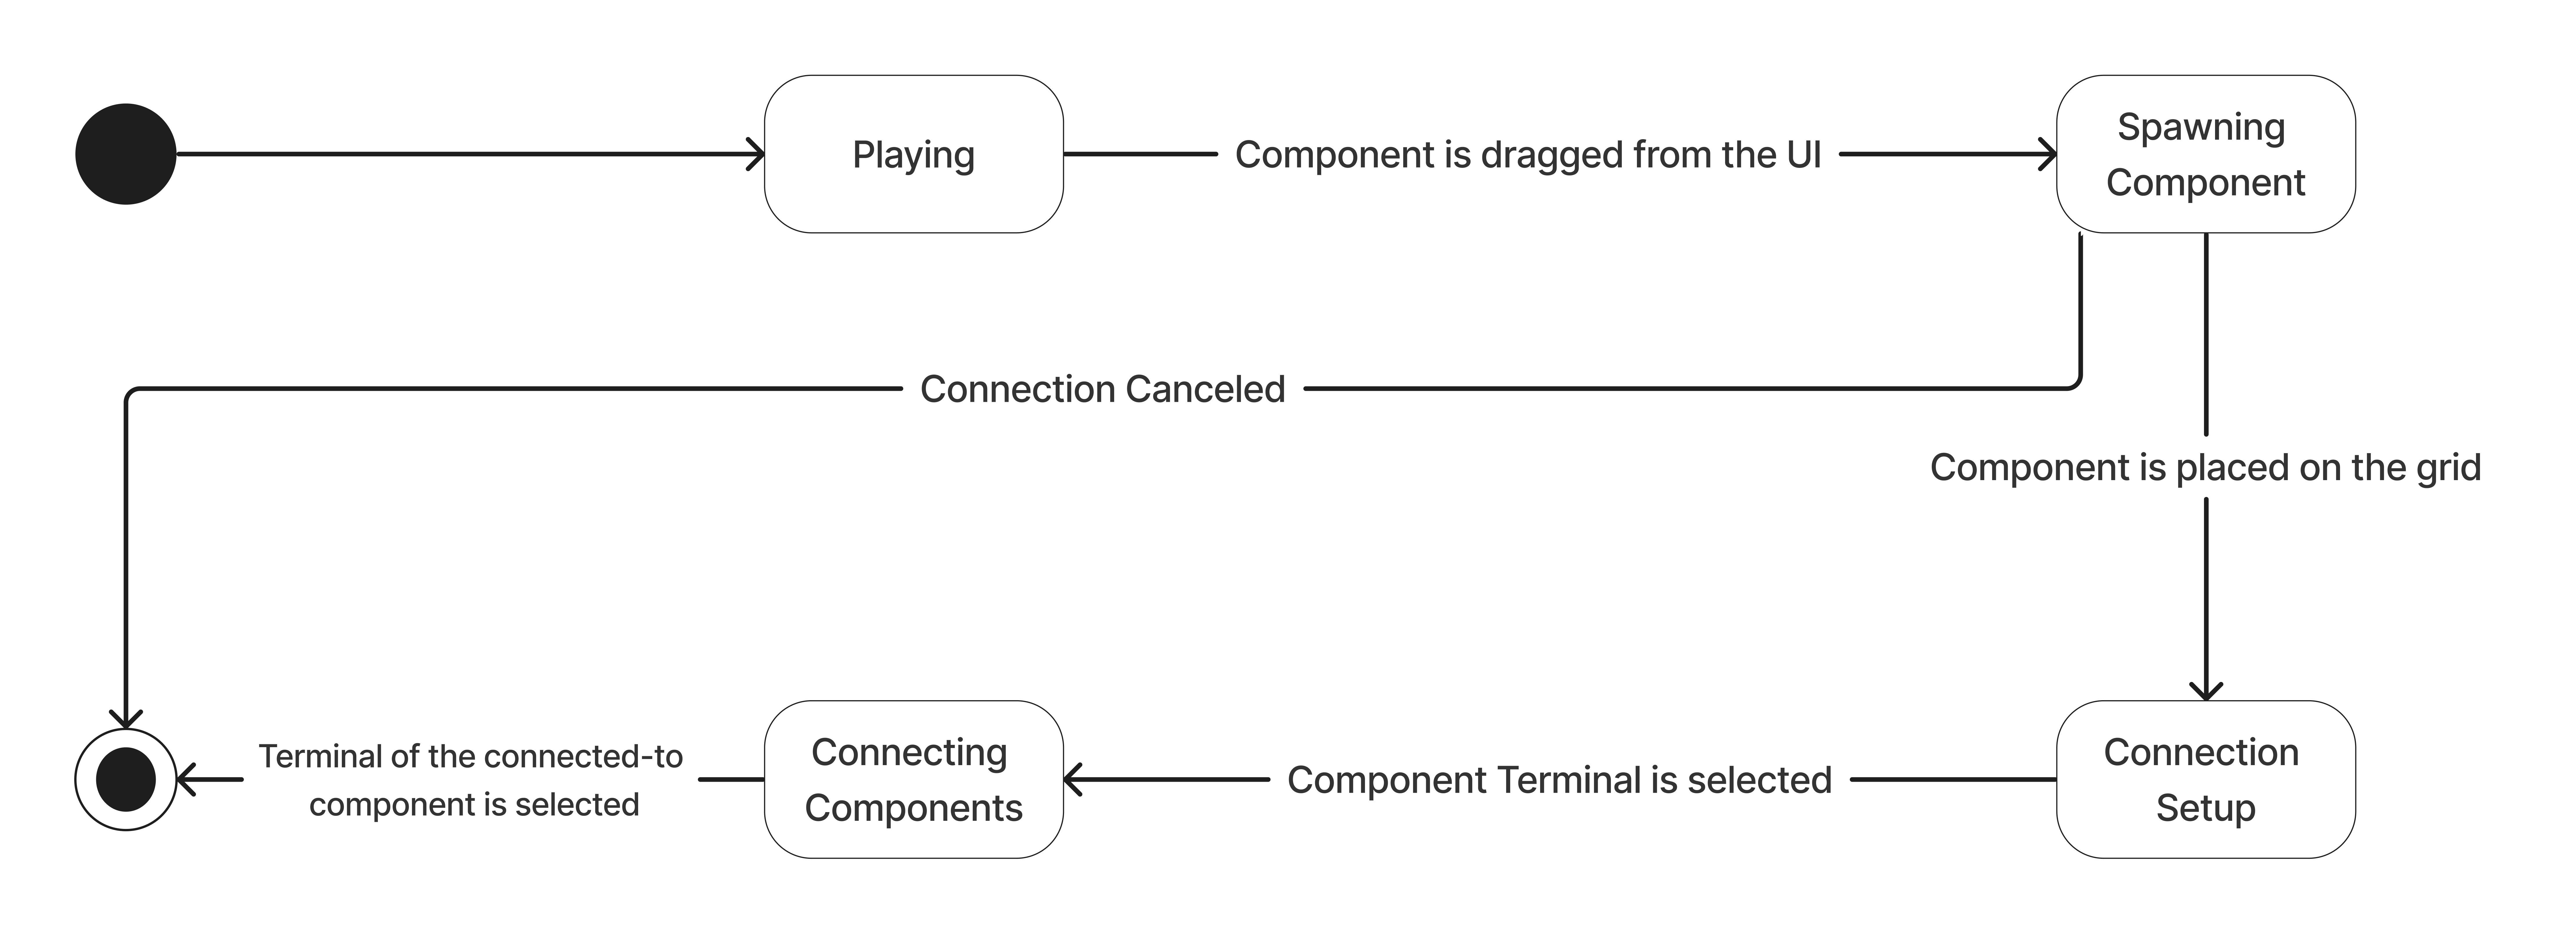
\includegraphics[scale=0.1]{images/chapter3/stateChart1.png}
\caption{Drag and Drop Components State Chart}
\label{Drag And Drop Components State Chart}
\end{figure}

\subsubsection{Simulate Circuits}
\begin{figure}[h!]
\centering
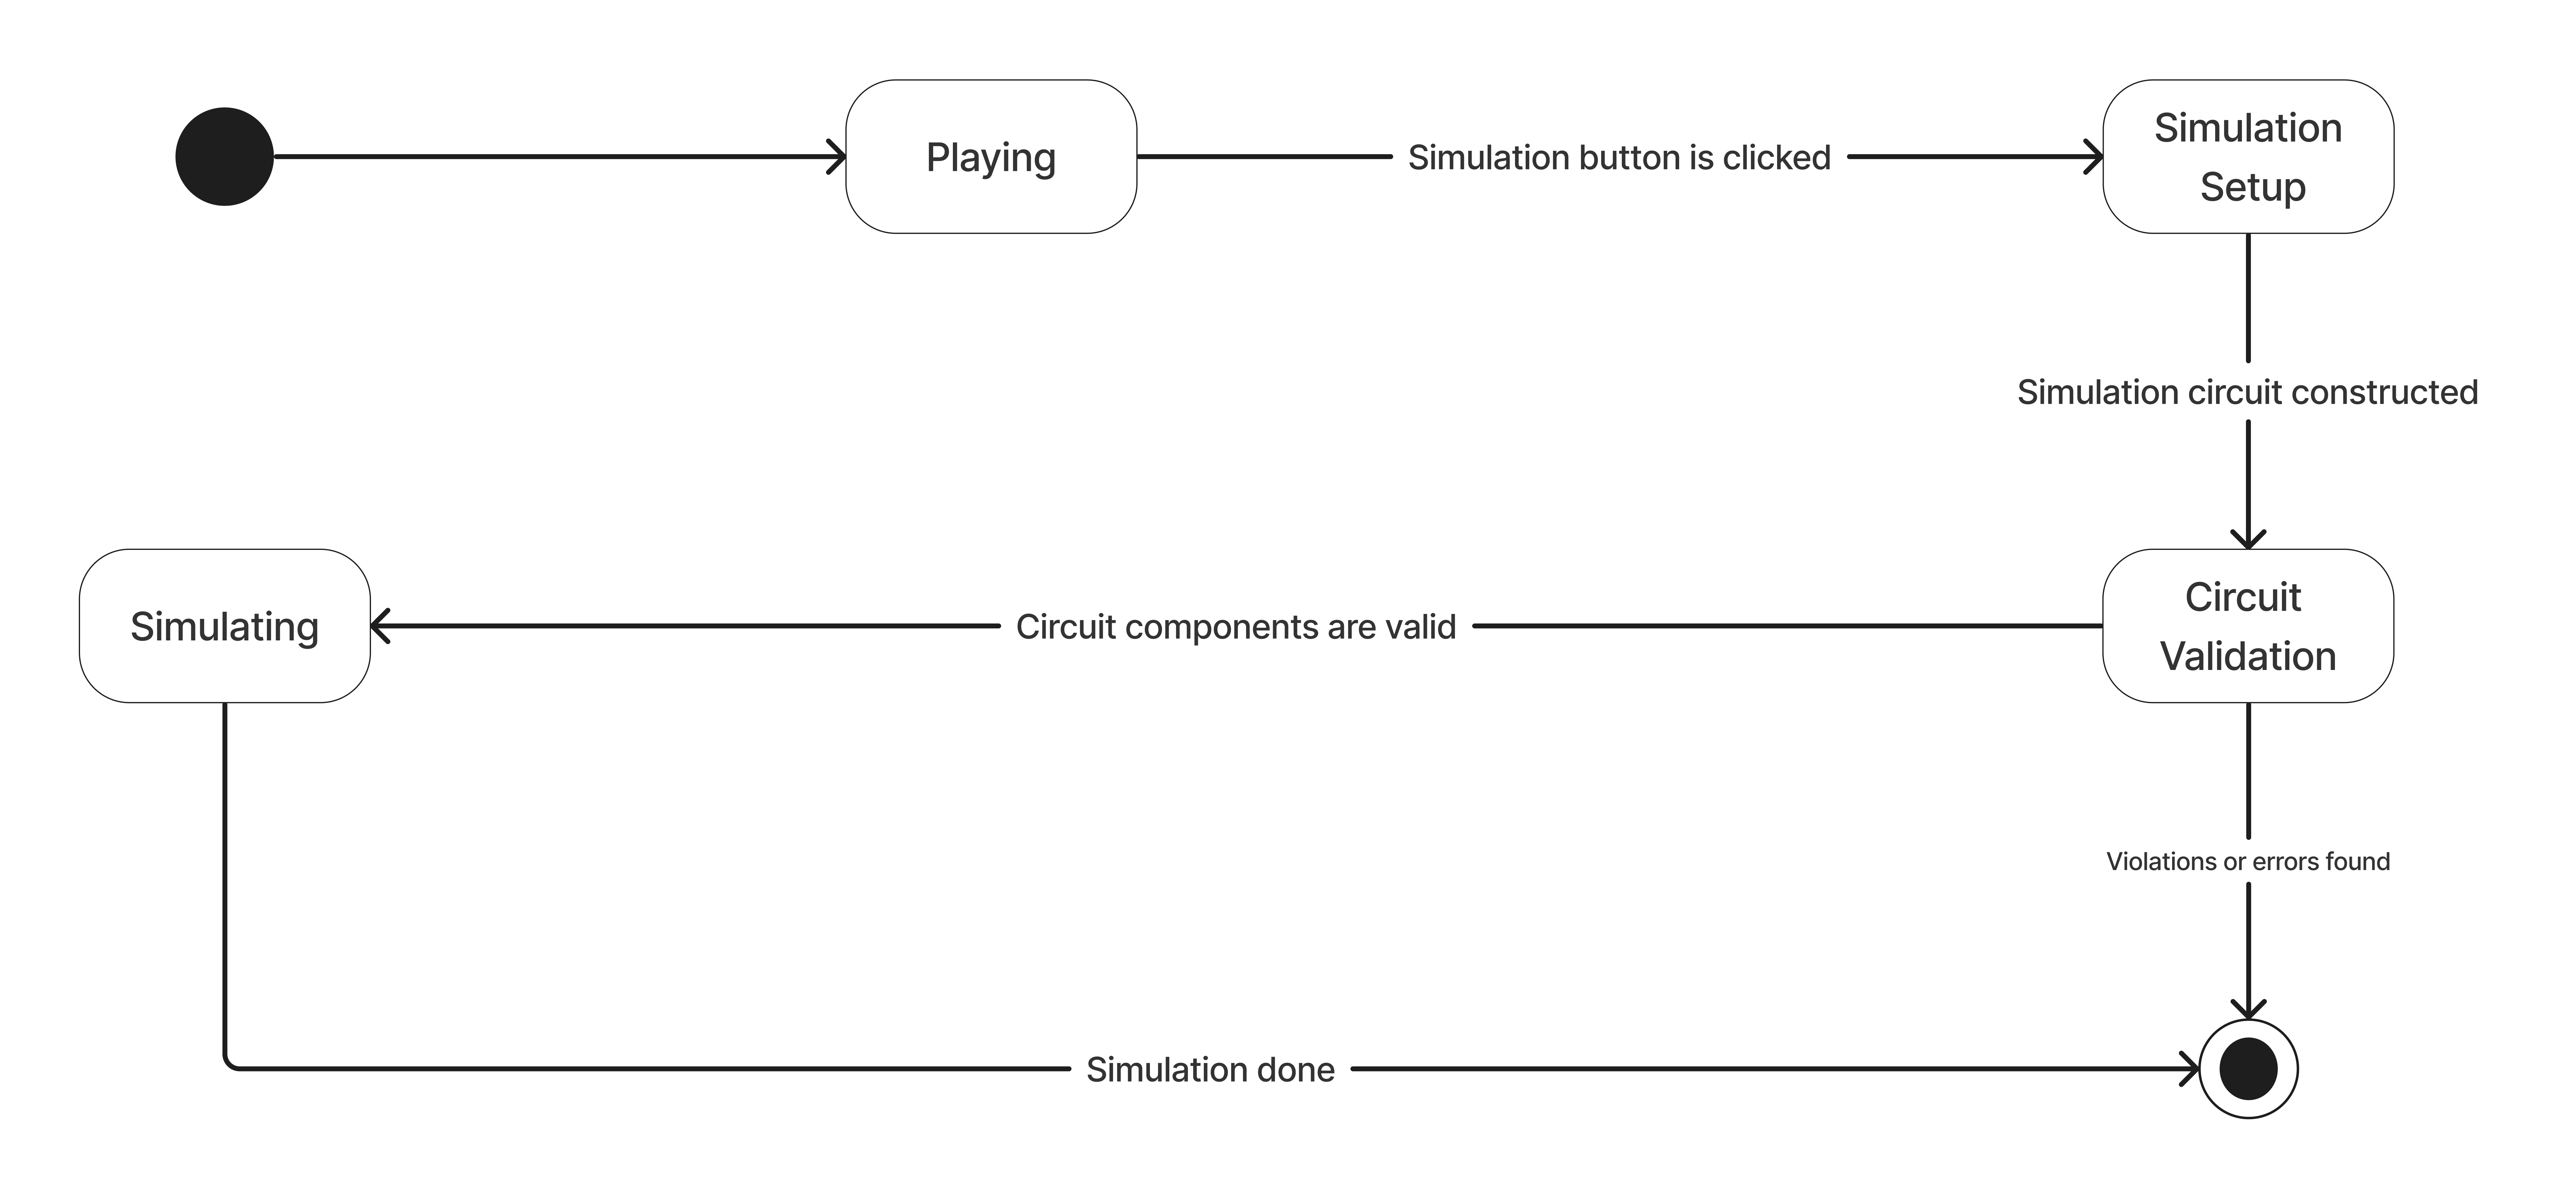
\includegraphics[scale=0.1]{images/chapter3/StateChart2.png}
\caption{Simulate Circuits State Chart}
\label{Simulate Circuits State Chart}
\end{figure}
\vfill
\newpage
\section{Methodologies}
\subsection{Software development life cycle (SDLC)}
\acrfull{sldc} is the process followed by developers when they are building a product. It consists of several phases, and each one is essential to the process of creating a high quality software. The life cycle describes the methodology the team follows in the overall development process. 
\subsubsection*{\underline{Stage 1: planning and requirement analysis
}}
This stage is the cornerstone for the whole process of building a software. In this stage, the planning for the system is done by the heads of the team, to define the project scope, set the goals and objectives of the system, and determine the risk associated with the project. The information collected is then used to plan the project approach. 
\subsubsection*{\underline{Stage 2: defining requirements
}} 
Once the first stage is done, a system analysis is conducted to determine and document the requirements of the system and get them approved by the stakeholders. Also, we will analyze the requirements to determine the characteristics of the system. 
\subsubsection*{\underline{Stage 3: designing the product architecture 
}} 
Based on the requirement specification, we will design the system architecture for the development process. Usually, more than one design is proposed and shown to the stakeholders to agree on which is the best one for the product. 
\subsubsection*{\underline{Stage 4: development
}}  
In this stage of the SDLC, the actual programming of the systems begins, based on the system architecture designed in the previous stage. The programmers should be able to develop the system without much hassle if the previous stages of development are done correctly. 
\subsubsection*{\underline{Stage 5: Testing
}} 
After the development is done, the system gets tested for bugs and errors, although testing is done simultaneously with every stage of the SDLC, in this stage the system is tested as a whole the reported bugs get fixed and re-tested.
\subsubsection*{\underline{Stage 6: Deployment 
}} 
Once the system is tested and ready to be published, it gets released in the market, sometimes a product will be deployed in stages and sometimes as a whole. After the deployment of the system and the users feedback, the product may receive updates to enhance the performance or fix any bugs found by the users. 

Although games are basically software, the SDLC is not suitable for game development, so we will follow \acrfull{gldc} in the making of this project. Which is more suited for game development. Also following methodologies like the waterfall model. 

\begin{figure}[!ht]
\centering
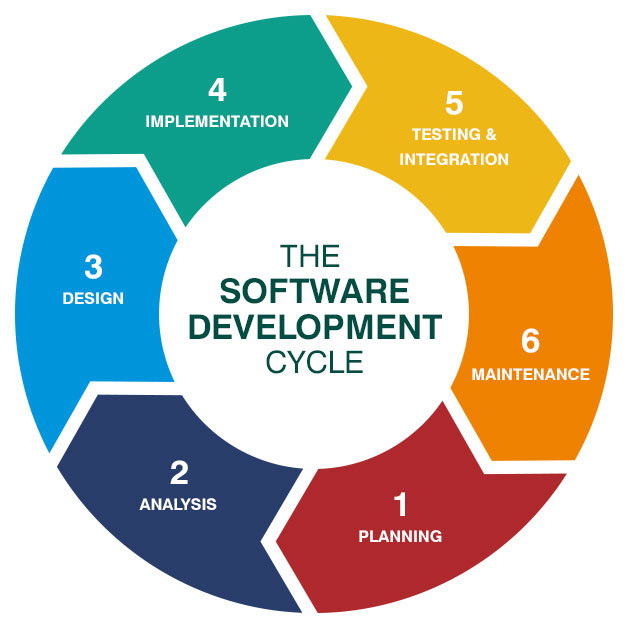
\includegraphics[scale=0.3]{images/chapter3/SDLC.png}
\caption{Software Development Life Cycle (SDLC)}
\label{sdlc}
\end{figure}
\newpage
\subsection{Game development stages and the game development life cycle (GDLC)}
Video games are in their essence software; depending on the scale of the game, project management and orchestration play a fundamental role in development. Games with poor project management are more likely to run over budget and time estimates, as well as contain a large number of bugs. However, unlike other kinds of software, games are not suitable for the typical software development life cycle (SDLC), but rather follow agile-like methodologies modified to suit the game development life cycle (GDLC), which goes roughly as follows for most games:
\subsubsection*{\underline{Pre-production stage}}
Also known as the planning phase (or both, combined into one stage), this is when the game’s initial and basic properties are specified. It is intended as a feasibility study of the game idea, followed by prototypes and documents, which can later be presented as proof-of-concept. This stage is mainly focused on idea and concept development, as well as documentation. Its goals are typically some or all of the following:
\begin{itemize}
    \item Develop and document game concepts, ideas, mechanics.
    \item Produce game descriptions and concept art.
    \item Write a proposal document if the game is to be sold to a publisher.
    \item Write a concept document, including comprehensive information such as:  the game's genre, gameplay description, features, setting, story, target audience, hardware platforms, estimated schedule, marketing analysis, team requirements, and risk analysis.
    \item Write a \acrfull{gdd} , a document which describes the game’s concept and major gameplay elements in detail. It may include concept art for the game, story plot, theme and colors, initial level design sketches, and may even be accompanied by a functional prototype for some of the game mechanics. This document is a living document, that is, the first version is produced in the pre-production stage, then the document is updated on weekly or even daily-basis during the production stage.
    \item Produce quick functional prototypes for select game mechanics.
\end{itemize}
\subsubsection*{\underline{Production stage}}
This is where the majority of the game’s development time, effort, and budget is spent. The entire development team is involved in this stage; artists, engineers, designers, musicians, writers, and many other talents will collaborate to bring the game together. This stage can take anywhere from a few months or less, to 10 or more years, depending on the scale of the game.
\subsubsection*{\underline{Testing stage}}
This stage most of the time does not fall in linear progression relative to the GDLC, but rather segments of the game go back and forth between production and testing. Test types vary and there are several game tester roles, varying from bug testing and stress testing, to gameplay, balance, and fun-factor testing. Several milestone releases of the game can go public during the production-testing cycle; alpha and beta versions of the game may go to public testing before the game moves to the next stage.

\subsubsection*{\underline{Launch stage}}
At this point, the game has been full-developed and tested, and is ready for the official launch. This stage is typically accompanied by game polishing, bug fixes, advertising and creating launch trailers and other publishing media, readying the game for launch and distribution.

\subsubsection*{\underline{Post-production stage}}
This stage involves bug fixes, game patches (balancing, minor content updates, etc…), and new content additions. New content might start off an entire new GDLC if it's large enough.



\begin{figure}[!ht]
\centering
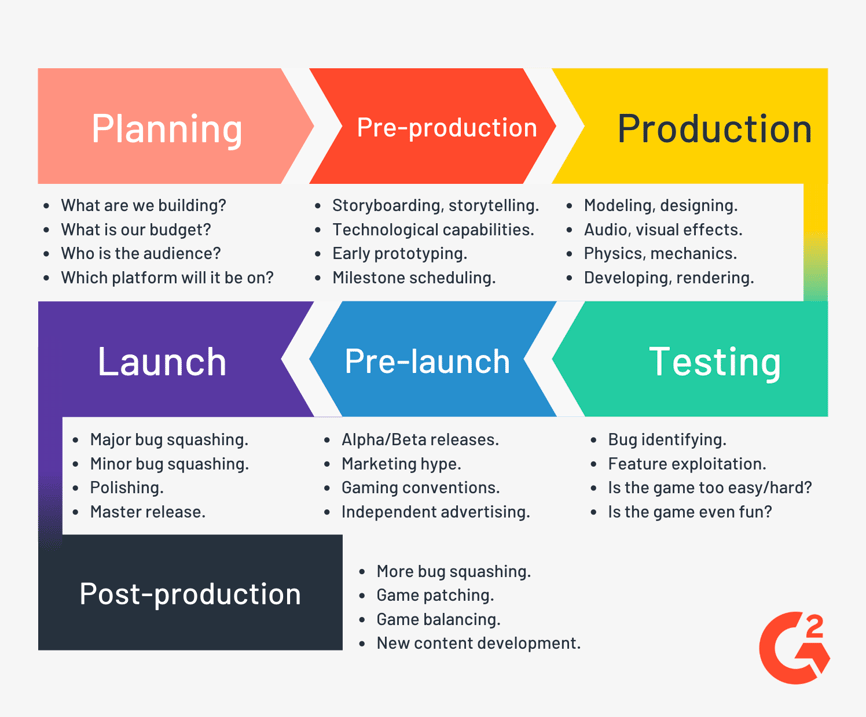
\includegraphics[scale=0.3]{images/chapter1/Example game development life cycle.png}
\caption{Example game development life cycle (GDLC) from G2}
\label{fig:Example game development life cycle (GDLC)}
\end{figure}
This stage involves bug fixes, game patches (balancing, minor content updates, etc…), and new content additions. New content might start off an entire new GDLC if it's large enough.
That all being said, an insightful research literature review (Aleem et al., 2016) \cite{11} also shows that despite the fact that a proper GDLC will help a game organization identify its strengths and weaknesses and provide guidance for improvement, the domain is still fragmented and lacks standard good practices relative to its typical SDLC counterpart. 
\newpage
\section{Algorithms}
\subsection{System Tools}
\subsubsection{Programming languages: }
\begin{itemize}
    \item C\#
\end{itemize}

\subsubsection{Frameworks:}
\begin{itemize}
    \item \underline{.NET framework:} .Net Framework is a software development platform for building and running Windows applications. The .Net framework consists of developer tools, programming languages, and libraries to build desktop and web applications. It is also used to build websites, web services, and games. 
\end{itemize}

\subsubsection{Tools:} 
\begin{itemize}
    \item \underline{Unity:} Unity is a cross-platform game engine developed by Unity Technologies used to build games. Unity provides game developers with a \acrshort{2d} and  \acrshort{3d} platform to create video games.
    \item \underline{SpiceSharp:} Circuit simulator used to simulate the results of each circuit in the levels. 
     \item \underline{Figma:} Used for designing the game UI and art.
      \item \underline{Git:} Git is a free and open source distributed version control system designed to handle everything from small to very large projects with speed and efficiency.
      \item \underline{IDEs:} Visual Studio Code 
\end{itemize}

\end{document}
